\chapter{0 文档控制信息}\label{ux6587ux6863ux63a7ux5236ux4fe1ux606f}

\section{0.1 术语、缩写与编号规则}\label{ux672fux8bedux7f29ux5199ux4e0eux7f16ux53f7ux89c4ux5219}

{\def\LTcaptype{none} % do not increment counter
\begin{xltabular}{\textwidth}{@{}>{\centering\arraybackslash}X>{\centering\arraybackslash}X@{}}
\toprule\noalign{}
\endhead
\bottomrule\noalign{}
\endlastfoot
\textbf{术语 / 缩写} & \textbf{说明} \\
结构化需求 &
用户发布需求时必须填写时间、地点、场景、人数、标签、要求等字段，使需求可筛选、可排序、可审核。 \\
信用摘要 &
根据互评、历史合作记录、举报与申诉结果形成的用户可靠性展示信息。 \\
P0 / P1 & 需求优先级。P0 为最小可用闭环必须实现，P1
为增强体验或扩展场景。 \\
MVP & Minimum Viable Product，最小可行产品，用于优先验证核心假设。 \\
编号规则 & 本文采用``英文前缀 +
序号''的编号方式，便于需求追踪、交叉引用和后续建模；编号仅用于定位需求条目，不代表实现顺序。 \\
RR & Raw Requirement /
原始问题需求编号，对应调研中归纳出的用户痛点或业务问题，例如 RR1。 \\
OBJ / KPI & 项目目标与成功指标编号，用于追踪目标和衡量方式，例如
OBJ-001、KPI-001。 \\
SF / MOD / IR &
系统特性、功能模块和研发需求编号，用于表示需求层级关系，例如
SF1、MOD-001、IR1。 \\
US / FR / AC &
用户故事、功能需求和验收标准编号，用于连接用户目标、功能描述和可验证结果，例如
US1、FR-001、AC-001。 \\
PAGE / UI & 页面与交互规则编号，用于定位界面清单和交互说明，例如
PAGE-001、UI-001。 \\
NFR & Non-functional Requirement /
非功能需求编号，按性能、安全、易用、兼容等类别区分，例如
NFR-SEC-002。 \\
OUT / ASM / DEP / RISK & 范围外内容、假设、依赖和风险编号，例如
OUT-001、ASM-001、DEP-001、RISK-001。 \\
\end{xltabular}
}

\chapter{1 项目概述}\label{ux9879ux76eeux6982ux8ff0}

\section{1.1 项目背景}\label{ux9879ux76eeux80ccux666f}

高校学生在日常学习和生活中存在持续、分散、高频的结伴需求。根据 125
份问卷，51.2\%
的学生在最近两周遇到``想找人一起做某件事，但找不到合适的人''的情况；58.4\%
的学生表示类似问题几乎每天或每周多次出现。访谈进一步显示，学生主要依赖宿舍群、班级群、朋友圈、校园墙和熟人介绍找人，但这些渠道存在消息被刷屏、无法筛选、回复滞后、伙伴不靠谱、主动联系陌生人有压力等问题。

本项目``校园搭子''旨在将零散、低效、依赖熟人的找人方式，转化为结构化发布、可筛选发现、低压力联系、信用沉淀的校内轻量匹配工具，使学生能够更快找到同时间、同地点、同目标、相对靠谱的结伴对象。


\begin{figure}[H]
\centering
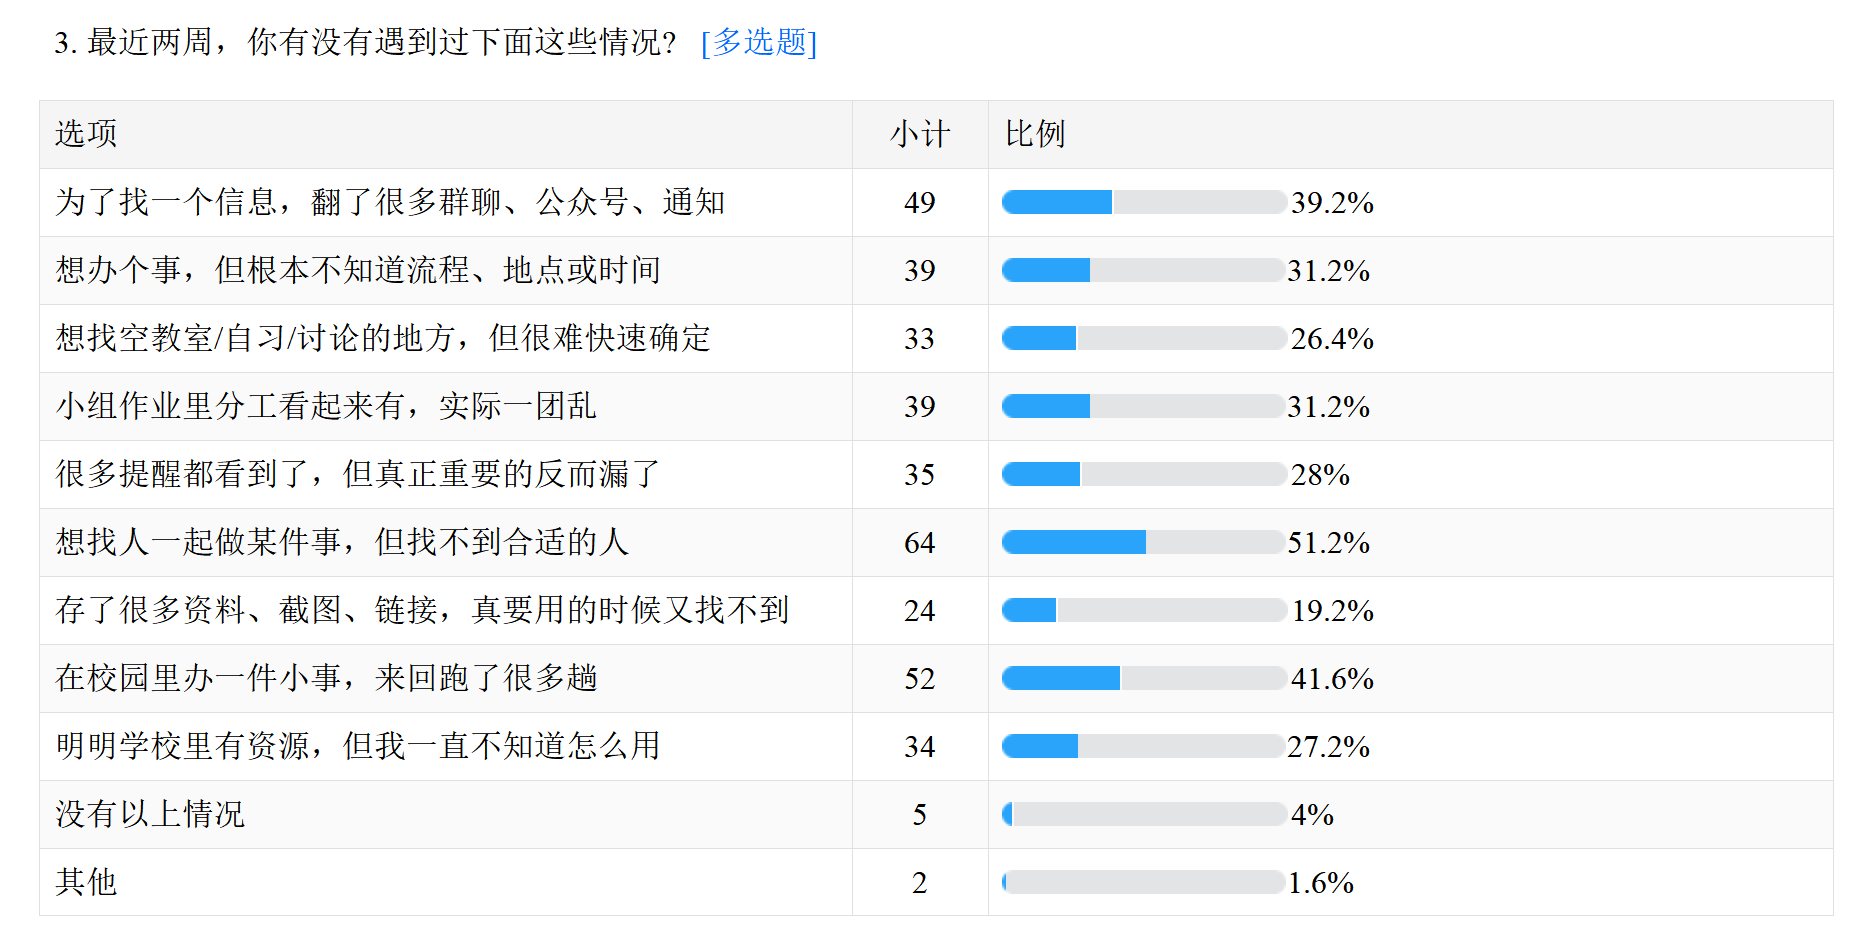
\includegraphics[width=0.96\textwidth,height=0.78\textheight,keepaspectratio]{picture/用户附件.png}
\vspace{0.4em}
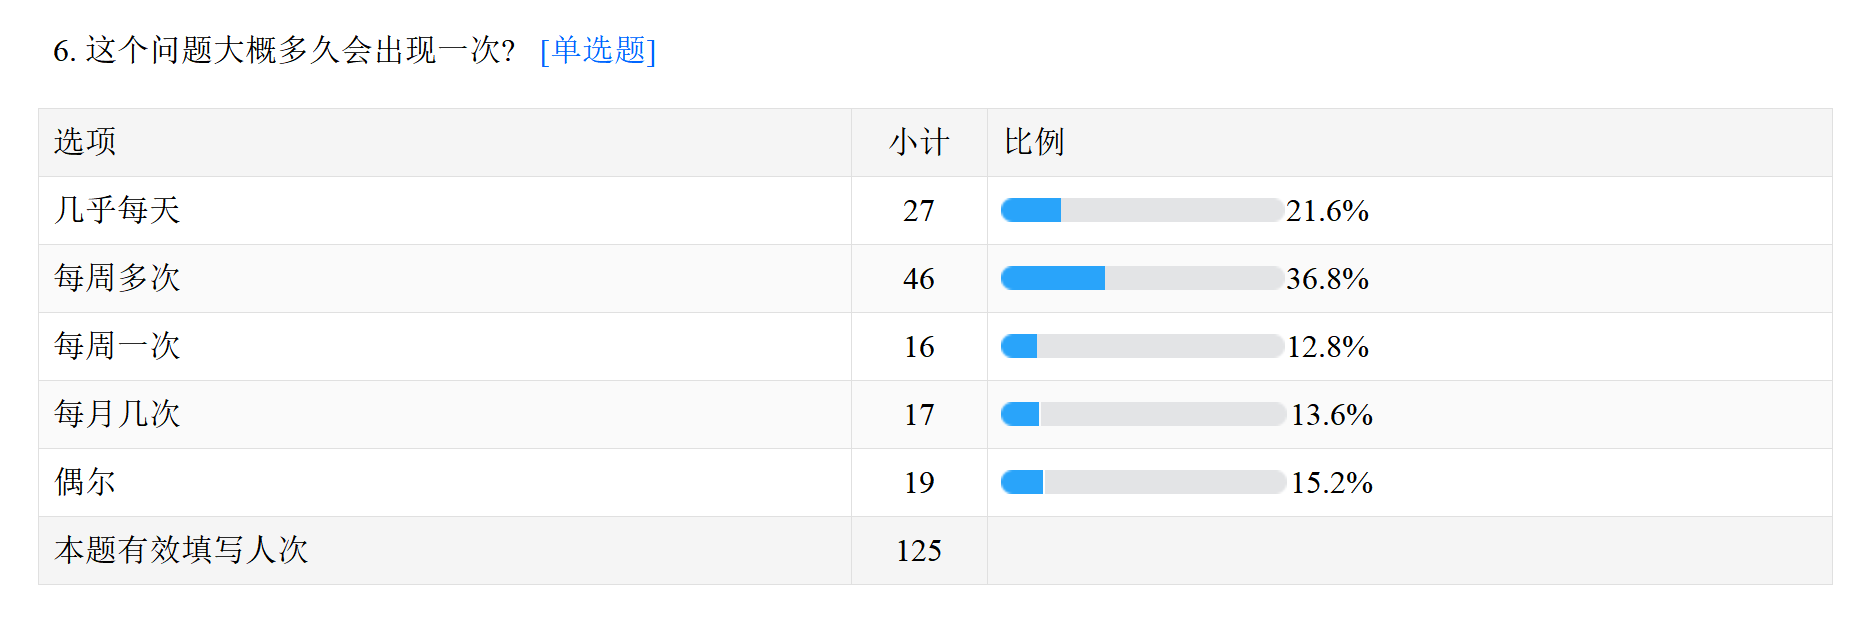
\includegraphics[width=0.96\textwidth,height=0.78\textheight,keepaspectratio]{picture/1-1.png}
\caption{图 1-1 问卷核心数据截图}
\end{figure}

\section{1.2 项目定位}\label{ux9879ux76eeux5b9aux4f4d}

校园搭子平台定位为``校内轻量级搭子匹配平台''。平台聚焦任务型、场景型连接，通过结构化信息和信用背书提升匹配效率。

\begin{itemize}
\item
  产品形态：面向单学校使用的校园搭子匹配软件。
\item
  核心对象：在校本科生与研究生。
\item
  核心场景：校内较广泛的搭子邀约场景如吃饭、学习、运动、项目队友招募等生活场景与学习场景。
\item
  核心能力：结构化发需求、广场筛选与推荐、邀约确认、站内低压力联系、互评与信用记录、基础治理。
\item
  非定位：不做完整即时通讯、不做跨校匹配、不做积分商城、不做支付担保、不做泛社交动态流。
\end{itemize}

\section{1.3 项目目标}\label{ux9879ux76eeux76eeux6807}

{\def\LTcaptype{none} % do not increment counter
\begin{xltabular}{\textwidth}{@{}>{\centering\arraybackslash}X>{\centering\arraybackslash}X>{\centering\arraybackslash}X>{\centering\arraybackslash}X>{\centering\arraybackslash}X@{}}
\toprule\noalign{}
\endhead
\bottomrule\noalign{}
\endlastfoot
\textbf{目标编号} & \textbf{目标类别} & \textbf{目标描述} &
\textbf{衡量方式 / 成功标准} & \textbf{优先级} \\
OBJ-001 & 效率目标 &
替代群聊刷屏和熟人转介绍方式，提升学生在校内寻找搭子的效率。 &
用户能够在 3 步内完成发布或发起邀约；平均找人耗时下降。 & 高 \\
OBJ-002 & 匹配目标 &
以时间、地点、标签、技能、水平、性别等字段为核心，提高需求发现和对象筛选准确性。
& MVP 阶段匹配成功率目标达到 60\%。 & 高 \\
OBJ-003 & 信任目标 &
通过身份认证、先审后发、互评信用和举报申诉降低爽约、失联、虚假信息风险。
& 形成可查询的评价、信用摘要和治理记录。 & 高 \\
OBJ-004 & 需求目标 & 形成可用于后续建模、方案设计与评审确认的需求基线。
& 需求可追踪到功能、用户故事和验收标准。 & 高 \\
\end{xltabular}
}

\section{1.4 项目价值}\label{ux9879ux76eeux4ef7ux503c}

{\def\LTcaptype{none} % do not increment counter
\begin{xltabular}{\textwidth}{@{}>{\centering\arraybackslash}X>{\centering\arraybackslash}X@{}}
\toprule\noalign{}
\endhead
\bottomrule\noalign{}
\endlastfoot
\textbf{价值对象} & \textbf{价值说明} \\
用户价值 &
降低找饭搭子、学习搭子、运动搭子和组队对象的时间成本与心理压力。 \\
业务价值 &
将分散在群聊、朋友圈和校园墙中的需求转为可筛选、可复用、可沉淀的数据。 \\
管理价值 &
通过审核、举报、申诉和账号处理形成基础治理能力，降低不良信息和纠纷风险。 \\
技术价值 & 为后续用例图、状态图、类图等软件建模活动提供统一需求边界。 \\
数据价值 &
沉淀场景、时间、地点、标签、评价等数据，为后续优化推荐规则提供依据。 \\
\end{xltabular}
}

\section{1.5 成功指标}\label{ux6210ux529fux6307ux6807}

{\def\LTcaptype{none} % do not increment counter
\begin{xltabular}{\textwidth}{@{}>{\centering\arraybackslash}X>{\centering\arraybackslash}X>{\centering\arraybackslash}X>{\centering\arraybackslash}X>{\centering\arraybackslash}X@{}}
\toprule\noalign{}
\endhead
\bottomrule\noalign{}
\endlastfoot
\textbf{指标编号} & \textbf{指标名称} & \textbf{指标说明} &
\textbf{目标值} & \textbf{统计方式} \\
KPI-001 & 匹配成功率 & 发布需求或发起邀约后成功建立搭子关系的比例。 &
MVP 目标 60\% & 系统记录发布、邀约、接受与关闭状态。 \\
KPI-002 & 流程步数 & 完成一次发布或邀约所需关键步骤。 & 不超过 3 步 &
可用性检查与界面流程统计。 \\
KPI-003 & 试用参与度 & 愿意参与原型试用或看情况参与的学生比例。 & 意愿组
47 人，潜在组 50 人 & 问卷第 16 题与后续招募记录。 \\
KPI-004 & 需求审核闭环率 &
提交需求经审核后明确进入通过或驳回状态的比例。 & 100\% 进入明确状态 &
后台审核记录。 \\
KPI-005 & 纠纷处理闭环率 & 举报、申诉案件被处理并留痕的比例。 & 100\%
进入明确状态 & 治理案件记录。 \\
\end{xltabular}
}

\chapter{2
业务背景与问题定义}\label{ux4e1aux52a1ux80ccux666fux4e0eux95eeux9898ux5b9aux4e49}

\section{2.1 调研基础}\label{ux8c03ux7814ux57faux7840}

本项目的需求来源包括：125 份校园真实需求问卷、12
次深度访谈、访谈纪要、需求评审演讲稿和已有需求分析报告草稿。问卷用于确定问题规模和优先级，访谈用于还原用户行为链路与痛点成因。

{\def\LTcaptype{none} % do not increment counter
\begin{xltabular}{\textwidth}{@{}>{\centering\arraybackslash}X>{\centering\arraybackslash}X>{\centering\arraybackslash}X>{\centering\arraybackslash}X@{}}
\toprule\noalign{}
\endhead
\bottomrule\noalign{}
\endlastfoot
\textbf{资料来源} & \textbf{样本 / 内容} & \textbf{主要结论} &
\textbf{用途} \\
问卷调查 & 125 份有效问卷 & 找人/找搭子困难在``最近两周遇到的问题''中占
51.2\%；``真能省时间''\,``打开就能解决问题''是长期使用工具的核心期待。 &
验证问题普遍性与工具价值标准。 \\
访谈 & 5 名 受访者 &
目前调研的找搭子具体场景如饭搭子、学习搭子、运动搭子、小组作业队友、大创队友等场景，存在相似链路：想找人、发消息、没人回应或不合适、最终放弃或低质量组队。
& 还原行为链路和具体需求字段。 \\
\end{xltabular}
}

\section{2.2 问题定义}\label{ux95eeux9898ux5b9aux4e49}

{\def\LTcaptype{none} % do not increment counter
\begin{xltabular}{\textwidth}{@{}>{\centering\arraybackslash}X>{\centering\arraybackslash}X>{\centering\arraybackslash}X>{\centering\arraybackslash}X@{}}
\toprule\noalign{}
\endhead
\bottomrule\noalign{}
\endlastfoot
\textbf{问题编号} & \textbf{问题定义} & \textbf{表现} & \textbf{影响} \\
RR1 & 现有找搭子渠道分散且触达效率低 &
群聊和校园墙刷屏快，消息被淹没，回复滞后。 &
用户错过时间窗口，最终一个人完成或放弃。 \\
RR2 & 缺少按条件筛选合适对象的能力 &
无法按时间、地点、水平、技能、作息、性别等筛选。 &
即使找到人，也可能不合适，反复沟通成本高。 \\
RR3 & 陌生人建立联系存在心理门槛 &
不好意思主动私聊陌生人，担心被拒绝或过早暴露联系方式。 &
潜在匹配无法发生，用户继续依赖熟人圈。 \\
RR4 & 缺少对爽约、划水、失联的识别与约束 &
随机组队中出现拖延、临时爽约、半途而废。 &
影响学习、运动和协作任务质量。 \\
RR5 & 历史合作关系无法沉淀复用 &
合作愉快的人无法被系统化记录和再次联系。 &
每次都重新筛选，无法形成稳定协作网络。 \\
RR6 & 平台缺少违规与纠纷治理抓手 &
虚假信息、骚扰、恶意评价、误处理缺少闭环。 &
用户信任下降，平台秩序不可控。 \\
\end{xltabular}
}
\begin{figure}[H]
\centering
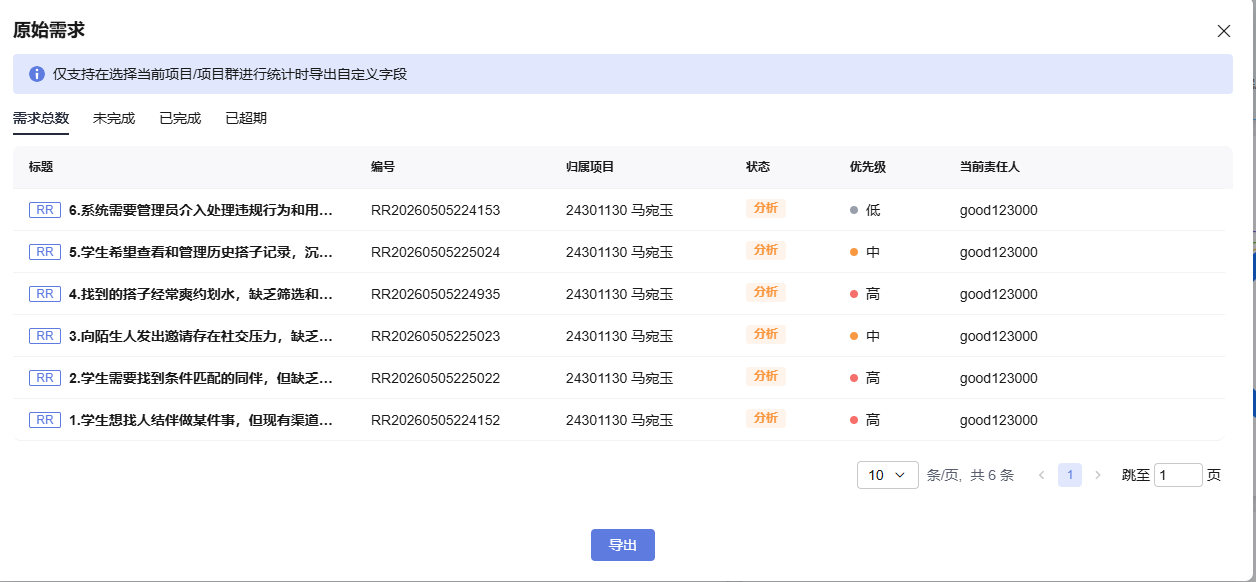
\includegraphics[width=0.96\textwidth,height=0.78\textheight,keepaspectratio]{picture/785092e90d6cbd4ba66ae0bac2c809f3.png}
\caption{图 6-1 原始需求截图}
\end{figure}


\section{2.3
核心问题归纳}\label{ux6838ux5fc3ux95eeux9898ux5f52ux7eb3}

综合问卷和访谈，学生并非没有找人的意愿，而是现有渠道效率低、失败率高。用户主要卡在两个环节：一是需求发出去但触达不到真正有空且有需求的人；二是触达后无法判断对方是否合适、是否靠谱。因此，本项目的核心问题可以概括为：如何让需求被看见、让人被筛选、让靠谱被记录。

\chapter{3
利益相关者与用户分析}\label{ux5229ux76caux76f8ux5173ux8005ux4e0eux7528ux6237ux5206ux6790}

\section{3.1 利益相关者}\label{ux5229ux76caux76f8ux5173ux8005}

{\def\LTcaptype{none} % do not increment counter
\begin{xltabular}{\textwidth}{@{}>{\centering\arraybackslash}X>{\centering\arraybackslash}X>{\centering\arraybackslash}X>{\centering\arraybackslash}X@{}}
\toprule\noalign{}
\endhead
\bottomrule\noalign{}
\endlastfoot
\textbf{角色} & \textbf{核心诉求} & \textbf{系统价值} &
\textbf{关注风险} \\
学生用户 & 快速找到合适搭子，降低找人和沟通成本。 &
平台主要服务对象，决定需求密度和活跃度。 &
匹配不到人、信息泄露、遇到不靠谱对象。 \\
被联系对象 & 筛选邀请，保护隐私，判断对方可靠性。 &
决定联系链路和转化效率。 & 被骚扰、被频繁打扰、被过早暴露联系方式。 \\
管理员 & 审核内容、处理举报和申诉、治理账号。 & 维持平台秩序和规则执行。
& 审核压力、误判、纠纷处理不透明。 \\
项目团队 & 统一需求基线，降低返工，形成可评审方案。 &
保障需求、建模和方案表达一致。 & 需求蔓延、范围不清、优先级混乱。 \\
\end{xltabular}
}

\section{3.2
目标用户画像}\label{ux76eeux6807ux7528ux6237ux753bux50cf}

{\def\LTcaptype{none} % do not increment counter
\begin{xltabular}{\textwidth}{@{}>{\centering\arraybackslash}X>{\centering\arraybackslash}X>{\centering\arraybackslash}X>{\centering\arraybackslash}X>{\centering\arraybackslash}X@{}}
\toprule\noalign{}
\endhead
\bottomrule\noalign{}
\endlastfoot
\textbf{画像} & \textbf{典型场景} & \textbf{核心诉求} &
\textbf{主要风险点} & \textbf{优先级} \\
P1 临时就餐型 & 饭点寻找同食堂饭搭子。 & 同时间、同地点、快速响应。 &
需求触达慢、消息被淹没。 & P0 \\
P2 学习陪伴型 & 备考、自习、监督学习。 & 目标一致、作息相近、可持续。 &
作息不匹配、长期稳定性差。 & P0 \\
P3 运动结伴型 & 羽毛球、跑步等运动搭子。 & 水平接近、地点合适、爽约少。
& 临时放鸽子、水平差异过大。 & P0 \\
P4 协作组队型 & 课程作业或大创项目组队。 & 技能匹配、责任心、可交付。 &
划水、拖延、能力失真。 & P1 \\
\end{xltabular}
}


\section{3.3
用户权限矩阵}\label{ux7528ux6237ux6743ux9650ux77e9ux9635}

{\def\LTcaptype{none} % do not increment counter
\begin{xltabular}{\textwidth}{@{}>{\centering\arraybackslash}X>{\centering\arraybackslash}X>{\centering\arraybackslash}X>{\centering\arraybackslash}X>{\centering\arraybackslash}X@{}}
\toprule\noalign{}
\endhead
\bottomrule\noalign{}
\endlastfoot
\textbf{功能 / 操作} & \textbf{未认证学生} & \textbf{已认证学生} &
\textbf{需求发布者} & \textbf{管理员} \\
浏览公开广场 & 允许 & 允许 & 允许 & 允许 \\
发布需求 & 禁止 & 允许 & 允许 & 允许 \\
编辑本人需求 & 禁止 & 允许本人编辑 & 允许本人编辑 & 可按治理规则处理 \\
发起邀约 & 禁止 & 允许 & 允许 & 允许 \\
查看联系方式 & 禁止 & 双方确认后允许 & 双方确认后允许 &
仅在治理需要时可查看必要信息 \\
提交评价 & 禁止 & 存在完成记录后允许 & 存在完成记录后允许 &
不参与评价 \\
举报 / 申诉 & 禁止 & 允许 & 允许 & 处理 \\
审核需求 & 禁止 & 禁止 & 禁止 & 允许 \\
冻结账号 & 禁止 & 禁止 & 禁止 & 允许 \\
\end{xltabular}
}

\chapter{4
业务范围与产品边界}\label{ux4e1aux52a1ux8303ux56f4ux4e0eux4ea7ux54c1ux8fb9ux754c}

\section{4.1
核心业务范围}\label{ux6838ux5fc3ux4e1aux52a1ux8303ux56f4}

\begin{itemize}
\item
  账号准入与身份校验：校园邮箱验证码登录，提交学号及基础校内信息完成认证。
\item
  结构化需求发布：按场景模板填写标题、时间、地点、人数、标签、能力/水平要求、补充描述。
\item
  内容审核：需求先进入待审核状态，管理员通过后进入公开广场。
\item
  广场发现：支持浏览、筛选、搜索、排序和规则推荐。
\item
  联系链路：支持邀约、双向确认、站内消息和联系方式渐进解锁。
\item
  评价沉淀：活动结束后互评，形成信用摘要和历史合作记录。
\item
  治理闭环：支持举报、申诉、被投诉方回应、管理员处理和账号限制。
\end{itemize}

\section{4.2
非本阶段范围}\label{ux975eux672cux9636ux6bb5ux8303ux56f4}

{\def\LTcaptype{none} % do not increment counter
\begin{xltabular}{\textwidth}{@{}>{\centering\arraybackslash}X>{\centering\arraybackslash}X>{\centering\arraybackslash}X>{\centering\arraybackslash}X@{}}
\toprule\noalign{}
\endhead
\bottomrule\noalign{}
\endlastfoot
\textbf{编号} & \textbf{非本阶段内容} & \textbf{原因} &
\textbf{后续计划} \\
OUT-001 & 完整即时通讯系统 &
问卷显示用户讨厌功能堆砌，且匹配后可使用微信等外部工具沟通。 &
仅保留站内低压力联系和联系方式渐进解锁。 \\
OUT-002 & 跨校匹配 &
本次调研场景均发生在校内，跨校会增加身份、距离和治理复杂度。 &
后续在单校模型稳定后再评估。 \\
OUT-003 & 积分商城和复杂运营体系 & 与核心找搭子问题关系弱，容易导致 MVP
失焦。 & 后续作为运营增强功能评估。 \\
OUT-004 & 支付、担保和交易撮合 &
本项目聚焦结伴和协作，不管理线下履约和资金交易。 & 暂不纳入。 \\
OUT-005 & 复杂算法推荐模型 & 当前阶段优先用规则筛选和排序验证需求。 &
数据积累后再考虑个性化算法。 \\
\end{xltabular}
}

\section{4.3
典型校园搭子邀约例子}\label{ux5178ux578bux6821ux56edux642dux5b50ux9080ux7ea6ux4f8bux5b50}

本项目覆盖的是较广泛的校内搭子邀约场景，包括但不限于就餐、学习、运动、课程协作、项目组队、活动同行、资源互助等。下表列出的五类场景是问卷与访谈中最具代表性的样例。

{\def\LTcaptype{none} % do not increment counter
\begin{xltabular}{\textwidth}{@{}>{\centering\arraybackslash}X>{\centering\arraybackslash}X>{\centering\arraybackslash}X>{\centering\arraybackslash}X>{\centering\arraybackslash}X@{}}
\toprule\noalign{}
\endhead
\bottomrule\noalign{}
\endlastfoot
典型场景样例 & \textbf{发布目的} & \textbf{关键字段} & 验证优先级 &
说明 \\
饭搭子 & 就餐结伴 & 时间段、食堂、预算、口味偏好、人数。 & P0 &
频次高、链路短，适合验证快速匹配能力。 \\
学习搭子 & 自习、备考、监督学习 &
学习目标、作息、频率、地点、监督方式、性别偏好。 & P0 &
稳定性需求强，适合验证作息、目标和信用匹配。 \\
运动搭子 & 运动结伴 & 运动项目、水平、场地、时间、人数、性别偏好。 & P0
& 筛选维度清晰，适合验证水平、场地和时间匹配。 \\
小组作业队友 & 课程作业组队 & 课程、角色、技能、交付周期、责任分工。 &
P1 & 作为协作类搭子邀约样例，用于观察责任分工和靠谱度需求。 \\
大创项目队友 & 项目协作 & 方向、角色、技能、投入周期、作品目标。 & P1 &
作为长期项目组队样例，用于观察技能、投入周期和责任心需求。 \\
\end{xltabular}
}

\section{4.4
需求优先级规则}\label{ux9700ux6c42ux4f18ux5148ux7ea7ux89c4ux5219}

{\def\LTcaptype{none} % do not increment counter
\begin{xltabular}{\textwidth}{@{}>{\centering\arraybackslash}X>{\centering\arraybackslash}X>{\centering\arraybackslash}X@{}}
\toprule\noalign{}
\endhead
\bottomrule\noalign{}
\endlastfoot
\textbf{优先级} & \textbf{含义} & \textbf{本项目应用} \\
Must / P0 & 必须实现，否则项目无法形成最小闭环。 &
账号认证、结构化发布、审核、广场筛选、邀约确认、基础互评。 \\
Should / P1 & 应实现，对体验和完整性重要，但可在 MVP 后完成。 &
站内消息增强、历史搭子再次联系、举报申诉闭环、P1 场景扩展。 \\
Could / P2 & 锦上添花，不影响核心流程验证。 &
个性化推荐、复杂标签运营、积分激励、活动发现。 \\
Won\textquotesingle t / 本期不做 & 明确不进入本期范围。 &
跨校、支付、完整 IM、积分商城、泛社交动态流。 \\
\end{xltabular}
}

\chapter{5
业务流程与用例分析}\label{ux4e1aux52a1ux6d41ux7a0bux4e0eux7528ux4f8bux5206ux6790}

\section{5.1
当前业务流程}\label{ux5f53ux524dux4e1aux52a1ux6d41ux7a0b}

以找饭搭子为例，当前流程通常为：饭点产生结伴需求，用户在宿舍群或微信私聊熟人，等待
15-20
分钟，因消息被刷屏或对方已吃过/没空导致无人回应，最终一个人吃饭或点外卖。学习、运动和组队场景也存在类似链路：先在群、朋友圈、校园墙发消息，再被动等待，最后因没人回应、不合适、不稳定而失败。

\section{5.2
目标业务流程}\label{ux76eeux6807ux4e1aux52a1ux6d41ux7a0b}

{\def\LTcaptype{none} % do not increment counter
\begin{xltabular}{\textwidth}{@{}>{\centering\arraybackslash}X>{\centering\arraybackslash}X>{\centering\arraybackslash}X>{\centering\arraybackslash}X@{}}
\toprule\noalign{}
\endhead
\bottomrule\noalign{}
\endlastfoot
\textbf{阶段} & \textbf{用户输入} & \textbf{系统处理} &
\textbf{输出结果} \\
账号准入 & 校园邮箱、验证码、基础身份信息 & 完成登录注册和认证状态记录 &
可用账号、认证状态。 \\
需求发布 & 场景类型、时间、地点、标签、描述、人数要求 &
校验字段完整性，提交审核 & 待审核需求。 \\
审核展示 & 管理员审核意见 & 通过、驳回或要求修改 &
公开需求或驳回结果。 \\
广场发现 & 搜索条件、筛选条件、排序条件 &
按时间、地点、标签、信用等规则筛选展示 & 候选需求或候选对象。 \\
联系确认 & 邀约、留言、站内消息 & 建立意向，双向确认后解锁联系方式 &
已确认关系或会话。 \\
合作完成 & 线下活动或线上协作结果 & 记录完成状态，触发评价入口 &
待评价关系。 \\
评价沉淀 & 准时性、合作态度、是否爽约等互评 & 更新信用摘要和历史记录 &
可供后续筛选的信任信息。 \\
\end{xltabular}
}


\section{5.3
管理侧治理流程}\label{ux7ba1ux7406ux4fa7ux6cbbux7406ux6d41ux7a0b}

{\def\LTcaptype{none} % do not increment counter
\begin{xltabular}{\textwidth}{@{}>{\centering\arraybackslash}X>{\centering\arraybackslash}X>{\centering\arraybackslash}X>{\centering\arraybackslash}X@{}}
\toprule\noalign{}
\endhead
\bottomrule\noalign{}
\endlastfoot
\textbf{阶段} & \textbf{输入} & \textbf{处理动作} & \textbf{输出} \\
内容审核 & 待审核需求 &
检查场景、标题、描述、联系方式、违规信息，选择通过或驳回。 &
公开需求或驳回结果。 \\
举报处理 & 用户举报、消息举报、需求举报 &
核验证据，选择警告、限制、冻结或驳回举报。 & 案件结果。 \\
申诉处理 & 申诉说明、证据、被投诉方回应 & 复核原处理结果，维持或纠正。 &
最终裁定。 \\
\end{xltabular}
}

\section{5.4 用例结构}\label{ux7528ux4f8bux7ed3ux6784}

需求分析阶段建议将用例图拆分为一个总体用例图和三个业务模块图。总体图描述学生用户、需求发布者、被联系对象、管理员与系统边界的关系；模块图分别覆盖需求发布与匹配、邀约与双向确认、信用评价与历史记录。


\clearpage
\begin{figure}[H]
\centering
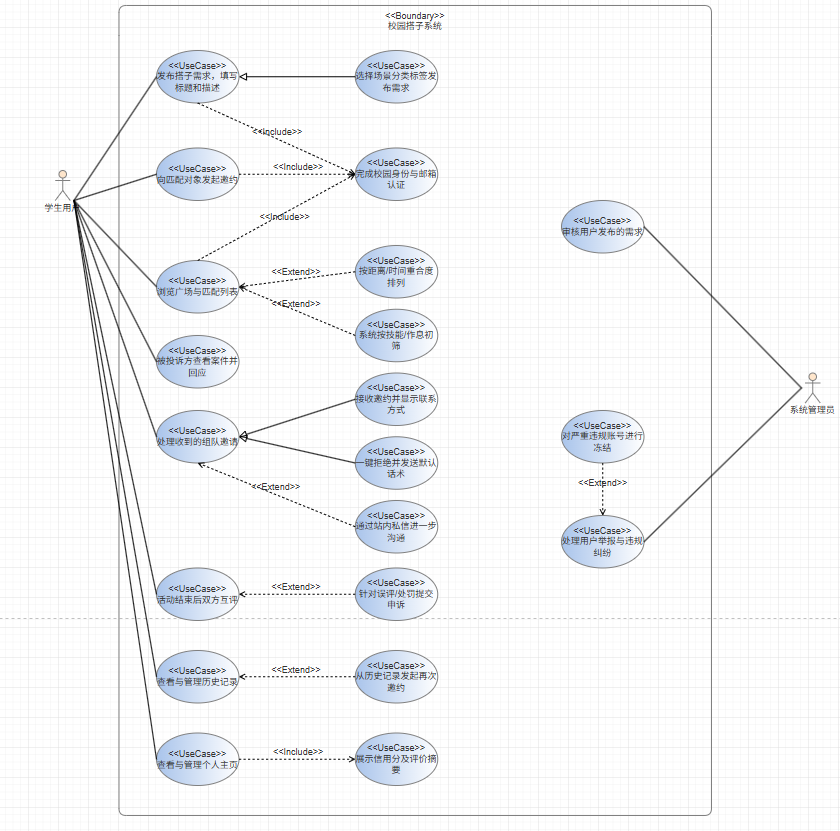
\includegraphics[width=0.96\textwidth,height=0.78\textheight,keepaspectratio]{picture/5-2.png}
\caption{图 5-2 总体用例图}
\end{figure}


\begin{figure}[H]
\centering
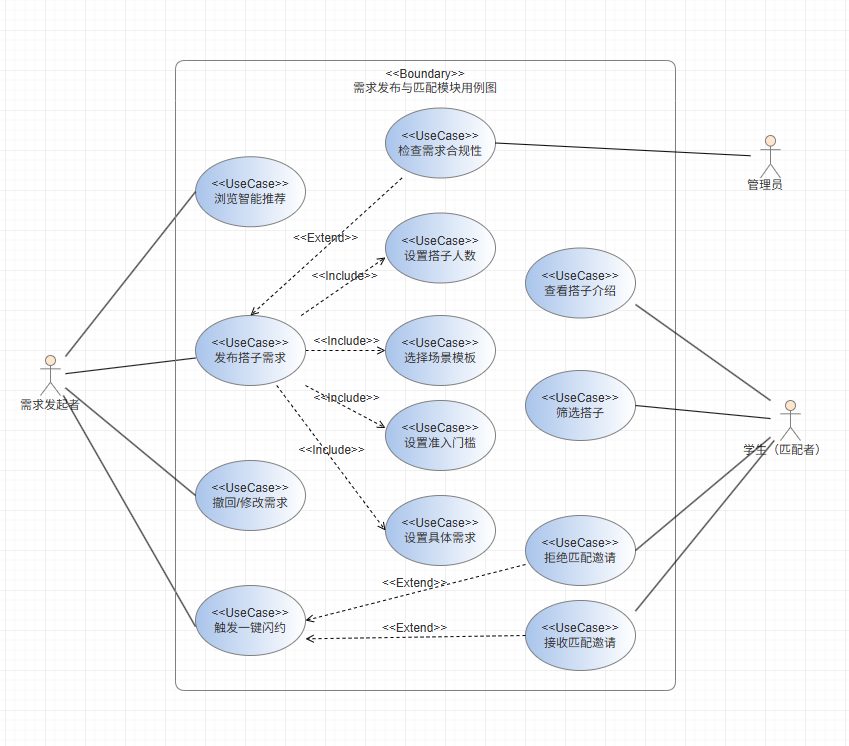
\includegraphics[width=0.96\textwidth,height=0.78\textheight,keepaspectratio]{picture/5-3.png}
\caption{图 5-3 模块用例图一：需求发布与匹配}
\end{figure}


\begin{figure}[H]
\centering
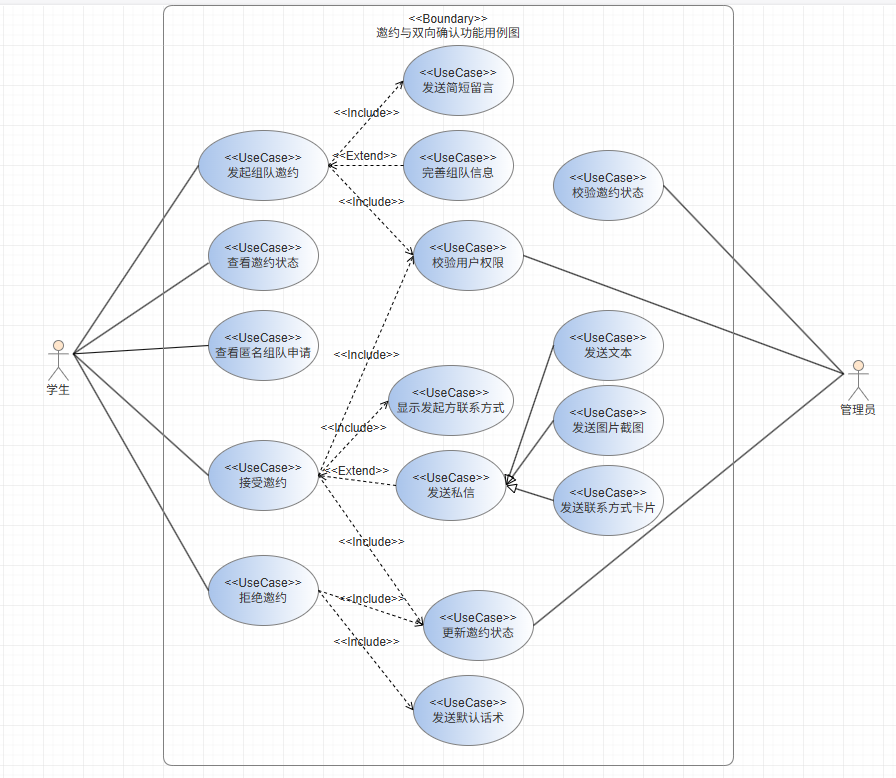
\includegraphics[width=0.96\textwidth,height=0.78\textheight,keepaspectratio]{picture/5-4.png}
\caption{图 5-4 模块用例图二：邀约与双向确认}
\end{figure}


\begin{figure}[H]
\centering
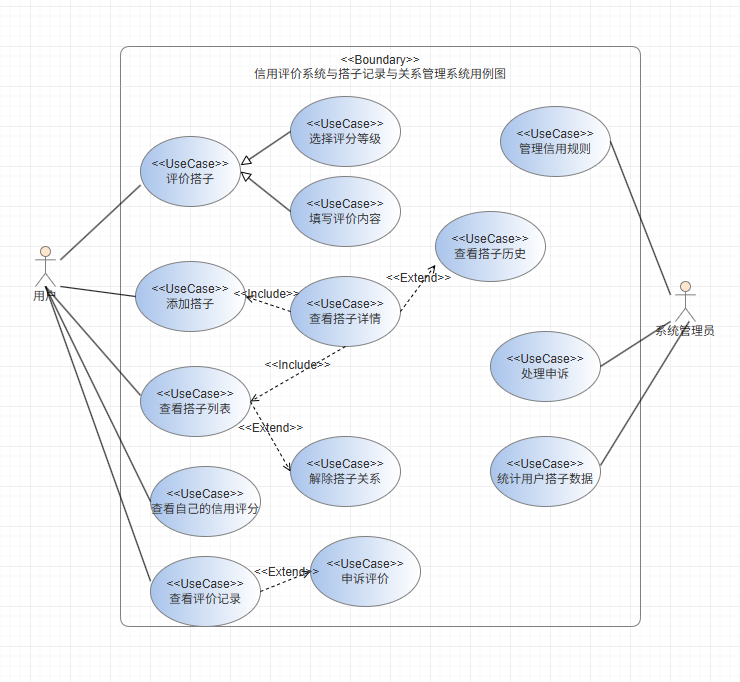
\includegraphics[width=0.96\textwidth,height=0.78\textheight,keepaspectratio]{picture/5-5.png}
\caption{图 5-5 模块用例图三：信用评价与历史记录}
\end{figure}
\clearpage

\chapter{6
需求分层与功能架构}\label{ux9700ux6c42ux5206ux5c42ux4e0eux529fux80fdux67b6ux6784}

\section{6.1
需求分层说明}\label{ux9700ux6c42ux5206ux5c42ux8bf4ux660e}

为保证需求可追踪，本项目在 CodeArts 工作项的需求管理中采用逐层分解的需求结构，而不是将 RR、SF、IR、US 作为互相并列的清单处理。整体逻辑是：先从调研和访谈中抽取原始需求（RR，Raw Requirement），明确用户痛点和业务问题；再将相近问题归并为系统特性（SF，System Feature），形成平台需要具备的能力域；随后把每个能力域细化为可开发、可验证的研发需求（IR，Initial Requirement）；最后从具体用户目标出发编写用户故事（US，User Story），并进一步连接验收标准。

因此，本章的阅读顺序应理解为``问题来源 → 能力归并 → 开发项拆解 → 用户场景表达''。RR 说明为什么要做，SF 说明系统要覆盖哪些能力，IR 说明这些能力需要落成哪些实现条目，US 则说明用户将在什么场景下使用这些能力。后续各表格中的``承接问题''、``所属系统特性''和``对应需求''字段，均用于维持这一层级关系，避免需求在编写和实现过程中失去来源。



\section{6.2 系统特性}\label{ux7cfbux7edfux7279ux6027}

在完成 RR 层的问题定义后，系统特性用于把分散的问题归并为相对稳定的能力域。同一个系统特性可以承接多个原始需求，一个原始需求也可能通过不同特性共同解决。表中``承接问题''字段用于说明每个 SF 从哪些 RR 推导而来，优先级则体现该能力域对核心问题的支撑程度。

{\def\LTcaptype{none} % do not increment counter
\begin{xltabular}{\textwidth}{@{}>{\centering\arraybackslash}X>{\centering\arraybackslash}X>{\centering\arraybackslash}X>{\centering\arraybackslash}X@{}}
\toprule\noalign{}
\endhead
\bottomrule\noalign{}
\endlastfoot
\textbf{系统特性} & \textbf{定义} & \textbf{承接问题} &
\textbf{优先级} \\
SF1 需求发布系统 & 承接结构化发布、字段校验、提交和进入审核队列。 &
RR1、RR2 & P0 \\
SF2 智能匹配与推荐系统 & 承接筛选、排序、推荐和广场发现。 & RR1、RR2 &
P0 \\
SF3 邀约与双向确认系统 & 承接低压力联系、邀约、站内消息和联系确认。 &
RR3 & P0/P1 \\
SF4 信用评价系统 & 承接互评、信用摘要、推荐权重影响和申诉纠偏。 &
RR4、RR6 & P1 \\
SF5 搭子记录与关系管理系统 &
承接历史记录、关系沉淀、再次联系和治理留痕。 & RR5、RR6 & P1 \\
SF6 平台治理系统 & 承接审核、举报、申诉、账号限制和处理留痕。 & RR6 &
P1 \\
\end{xltabular}
}


\begin{figure}[H]
\centering
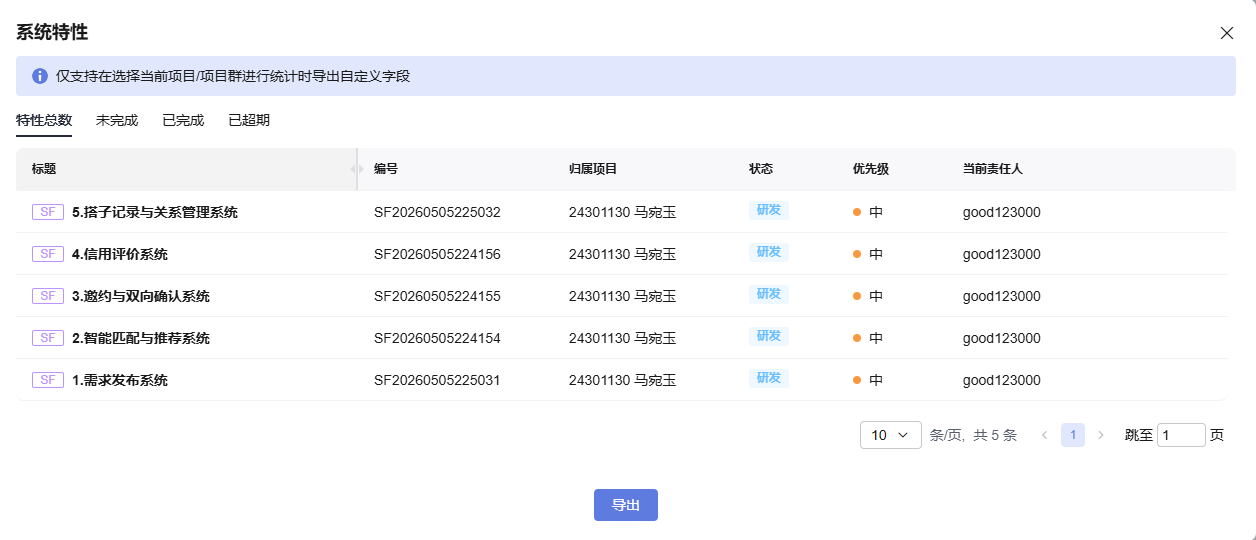
\includegraphics[width=0.96\textwidth,height=0.78\textheight,keepaspectratio]{picture/e9063c6533924a0086e104c235025ee6.png}
\caption{图 6-2 系统特性截图}
\end{figure}

\section{6.3
功能模块总览}\label{ux529fux80fdux6a21ux5757ux603bux89c8}

系统特性确定后，需要进一步落到产品与系统边界上。功能模块不是新的需求层级，而是对 SF 的工程化组织方式：它把能力域拆成可设计、可分工、可实现的模块，便于后续将研发需求挂接到具体模块和功能结构中。

{\def\LTcaptype{none} % do not increment counter
\begin{xltabular}{\textwidth}{@{}>{\centering\arraybackslash}X>{\centering\arraybackslash}X>{\centering\arraybackslash}X>{\centering\arraybackslash}X>{\centering\arraybackslash}X@{}}
\toprule\noalign{}
\endhead
\bottomrule\noalign{}
\endlastfoot
\textbf{模块编号} & \textbf{模块名称} & \textbf{模块说明} &
\textbf{包含功能} & \textbf{优先级} \\
MOD-001 & 账号与身份认证 & 保证使用者为校内学生，并建立权限边界。 &
邮箱登录、验证码、基础资料、认证状态。 & P0 \\
MOD-002 & 需求发布与审核 &
将找搭子需求转为结构化、可审核、可展示的数据。 &
发布、草稿、校验、审核、驳回、修改。 & P0 \\
MOD-003 & 广场发现与筛选 & 让用户快速浏览和筛选合适需求或对象。 &
列表、搜索、筛选、排序、规则推荐。 & P0 \\
MOD-004 & 邀约与联系确认 & 在低压力状态下建立初步联系和双向确认。 &
邀约、接受、拒绝、匿名展示、站内消息、联系方式解锁。 & P0/P1 \\
MOD-005 & 评价与信用 & 沉淀准时性、合作态度、是否爽约等信任信息。 &
互评、信用摘要、评价申诉。 & P1 \\
MOD-006 & 举报申诉与治理 & 处理违规、骚扰、虚假信息、误评和纠纷。 &
举报、案件处理、申诉、回应、账号限制。 & P1 \\
\end{xltabular}
}

\section{6.4 功能结构树}\label{ux529fux80fdux7ed3ux6784ux6811}

系统名称：校园搭子平台\\
├── 账号与身份认证\\
│ ├── 校园邮箱验证码登录\\
│ ├── 基础资料填写\\
│ └── 校内身份认证\\
├── 需求发布与审核\\
│ ├── 结构化需求发布\\
│ ├── 草稿与编辑\\
│ ├── 需求审核\\
│ └── 需求关闭\\
├── 广场发现与筛选\\
│ ├── 需求列表\\
│ ├── 场景筛选\\
│ ├── 时间/地点/标签筛选\\
│ └── 规则排序与推荐\\
├── 邀约与联系确认\\
│ ├── 发起邀约\\
│ ├── 接受/拒绝邀约\\
│ ├── 站内消息\\
│ └── 联系方式解锁\\
├── 评价与信用\\
│ ├── 活动完成确认\\
│ ├── 双方互评\\
│ ├── 信用摘要\\
│ └── 评价申诉\\
└── 平台治理\\
├── 举报处理\\
├── 申诉复核\\
├── 账号限制\\
└── 处理留痕

\section{6.5
研发需求总览}\label{ux7814ux53d1ux9700ux6c42ux603bux89c8}

在 SF 明确系统能力边界后，IR 层将这些能力进一步拆解为开发团队可以实现和验证的需求条目。IR 不再描述抽象问题，而是描述系统应提供的功能、规则或处理机制；表中``所属系统特性''字段用于说明每条 IR 回溯到哪个能力域，从而保持从 RR 到 SF 再到 IR 的追踪链。

{\def\LTcaptype{none} % do not increment counter
\begin{xltabular}{\textwidth}{@{}>{\centering\arraybackslash}X>{\centering\arraybackslash}X>{\centering\arraybackslash}X>{\centering\arraybackslash}X@{}}
\toprule\noalign{}
\endhead
\bottomrule\noalign{}
\endlastfoot
\textbf{编号} & \textbf{研发需求} & \textbf{所属系统特性} &
\textbf{优先级} \\
IR1 & 用户可以创建搭子需求，填写标题和详细描述。 & SF1 & P0 \\
IR2 &
发布需求时支持选择吃饭、学习、运动、小组作业、大创项目等典型场景标签，并支持其他校园搭子邀约场景。
& SF1 & P0 \\
IR3 & 发布需求时支持设置时间信息和紧急程度。 & SF1 & P0 \\
IR4 & 发布需求时支持设置地点和人数上限。 & SF1 & P0 \\
IR5 & 系统根据需求标签、时间和地点筛选条件相近的其他用户或需求。 & SF2 &
P0 \\
IR6 & 匹配结果可按时间重合度排序展示。 & SF2 & P0 \\
IR7 & 匹配结果可按地点或距离近似度排序展示。 & SF2 & P0 \\
IR8 & 用户可向匹配对象发起组队意向并附带简短留言。 & SF3 & P0 \\
IR9 &
接收方看到邀请时对方信息可先匿名或半匿名展示，接受后再显示联系方式。 &
SF3 & P0 \\
IR10 & 支持一键拒绝并附带默认话术，拒绝后双方互不可见或减少打扰。 & SF3
& P1 \\
IR11 & 搭子活动结束后双方互评，评价维度包含准时性、合作态度和是否爽约。
& SF4 & P1 \\
IR12 & 用户个人主页展示信用分和近期评价摘要。 & SF4 & P1 \\
IR13 & 低信用分用户在匹配推荐中降低权重。 & SF4 & P1 \\
IR14 & 用户可以查看历史搭子记录列表。 & SF5 & P1 \\
IR15 & 管理员可查看和处理用户举报。 & SF6 & P1 \\
IR16 & 管理员可对违规账号进行限制或冻结处理。 & SF6 & P1 \\
IR17 & 用户可通过校园邮箱验证码完成登录或注册。 & SF1 & P0 \\
IR18 & 用户需提交学号及基础校内信息完成身份认证。 & SF1 & P0 \\
IR19 & 搭子需求提交后需经管理员审核通过方可进入广场。 & SF1/SF6 & P0 \\
IR20 & 用户可通过站内消息发送文本、截图和联系方式卡片。 & SF3 & P1 \\
IR21 & 用户可针对评价、举报处理或纠纷结果提交申诉并上传证据。 & SF4/SF6
& P1 \\
IR22 & 被投诉方可查看案件并补充说明与证据回应。 & SF6 & P1 \\
\end{xltabular}
}


\begin{figure}[H]
\centering
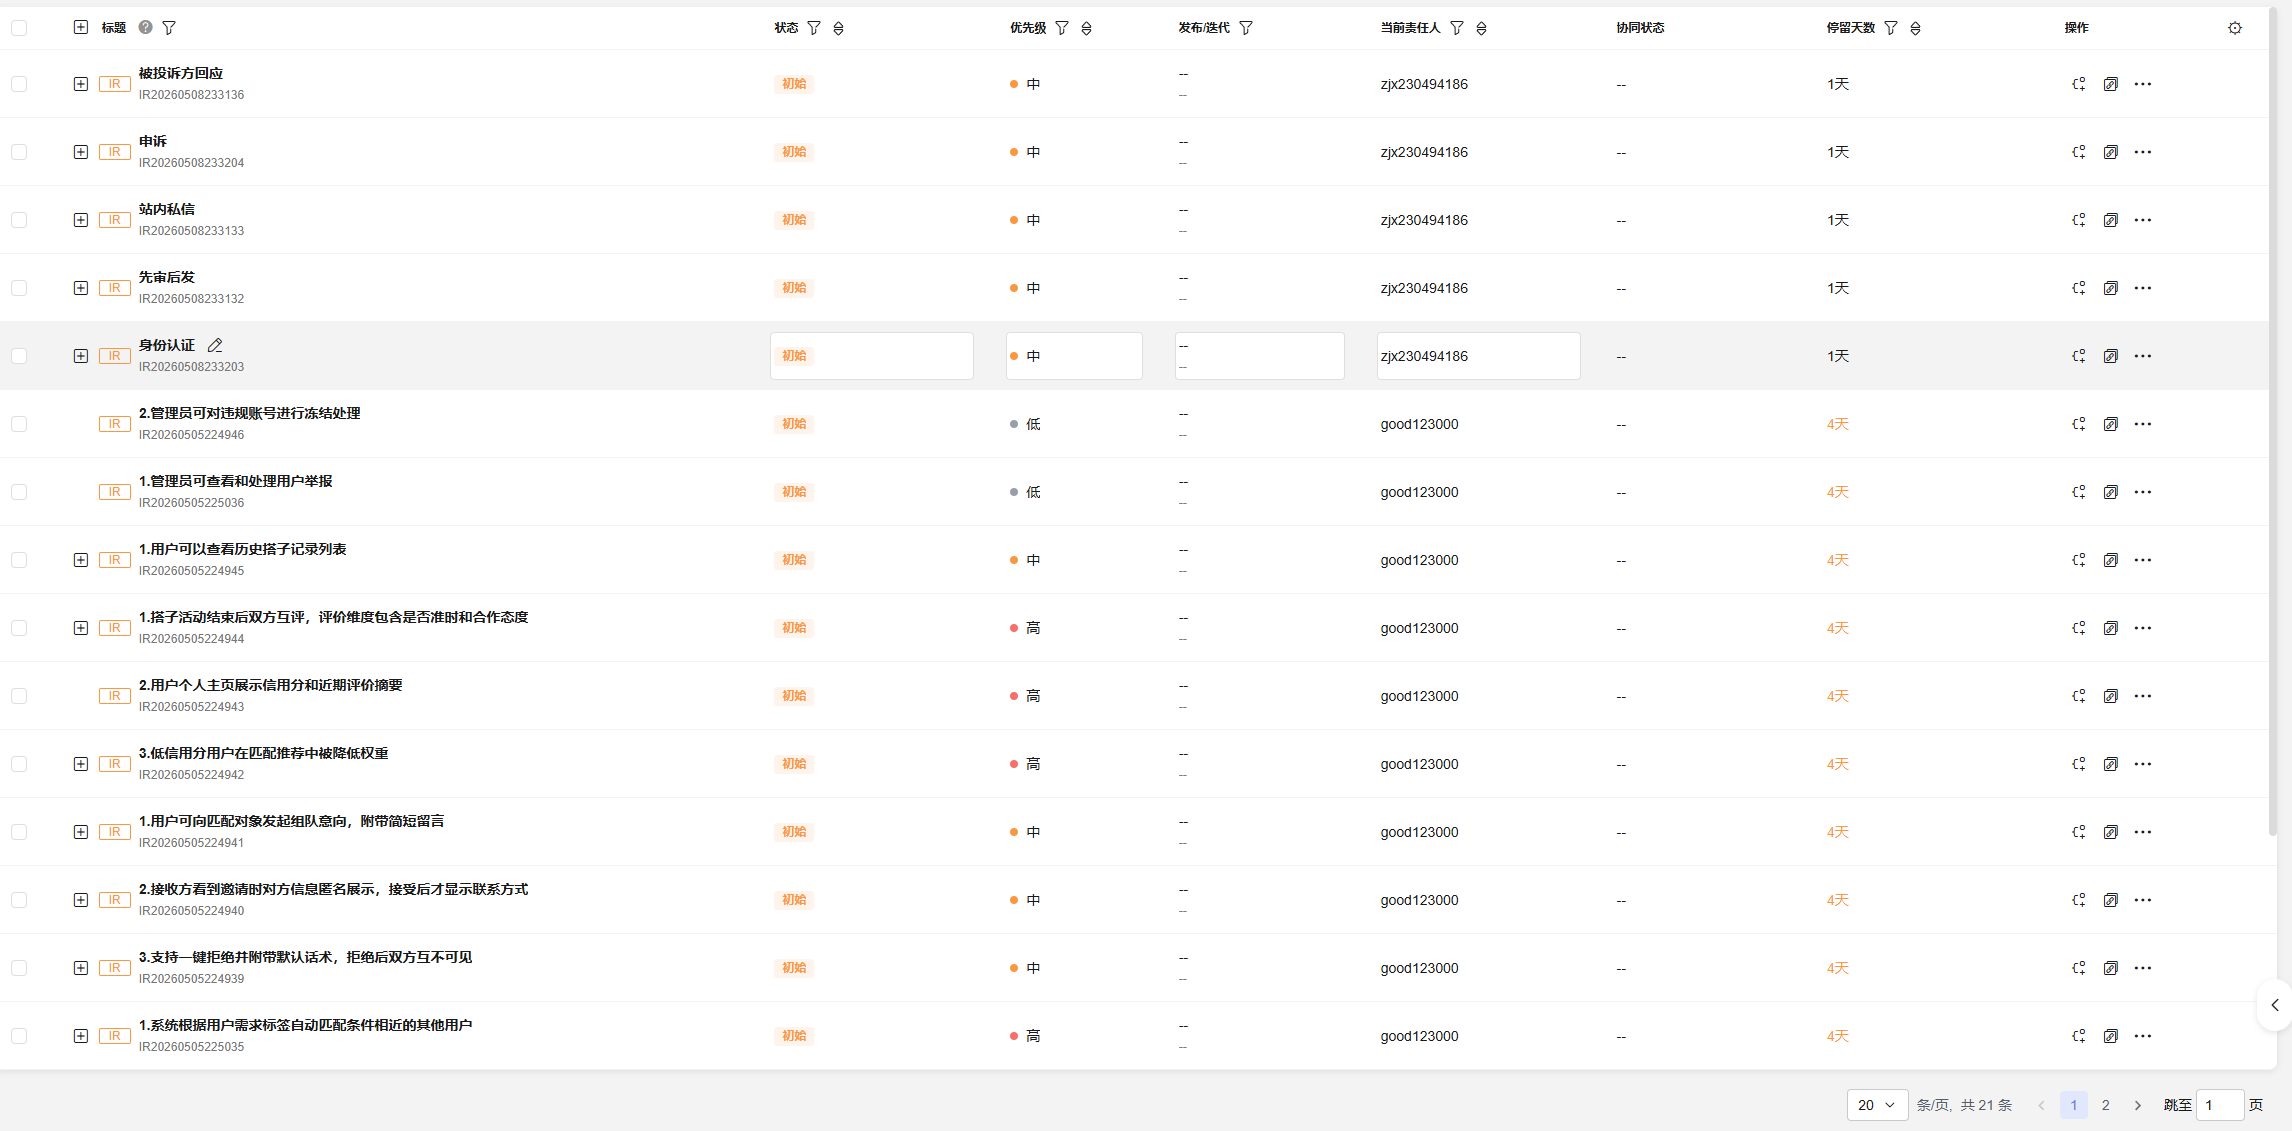
\includegraphics[width=0.96\textwidth,height=0.78\textheight,keepaspectratio]{picture/6-3.png}
\caption{图 6-3 研发需求截图}
\end{figure}

\section{6.6
用户故事总览}\label{ux7528ux6237ux6545ux4e8bux603bux89c8}

用户故事用于把 IR 转换为用户视角下的目标、动机和收益表达。它不是对 IR 的重复罗列，而是说明具体角色为什么需要这些功能、在什么场景下使用这些功能，以及功能完成后应带来什么结果。表中``对应需求''字段用于把 US 与 IR 连接起来，后续验收标准可继续围绕这些用户故事展开。

{\def\LTcaptype{none} % do not increment counter
\begin{xltabular}{\textwidth}{@{}>{\centering\arraybackslash}X>{\centering\arraybackslash}X>{\centering\arraybackslash}X>{\centering\arraybackslash}X@{}}
\toprule\noalign{}
\endhead
\bottomrule\noalign{}
\endlastfoot
\textbf{编号} & \textbf{用户故事} & \textbf{优先级} &
\textbf{对应需求} \\
US1 &
作为饭点想结伴的学生，我希望快速匹配同时间、同食堂的饭搭子，以便不用长时间等群消息回复。
& 高 & IR1-IR8 \\
US2 &
作为发布需求的学生，我希望我的需求被真正有空的人稳定看到，以便不再被群聊刷屏淹没。
& 高 & IR1、IR19 \\
US3 &
作为备考学生，我希望按学习目标和作息时间匹配固定学伴，以便长期互相监督。
& 高 & IR1-IR7 \\
US4 & 作为用户，我希望提前识别并避开经常爽约的对象，以便降低试错成本。 &
高 & IR11-IR13 \\
US5 &
作为运动爱好者，我希望按运动水平、时间和场地筛选运动伙伴，以便找到合适球友。
& 中 & IR1-IR7 \\
US6 &
作为运动需求发布者，我希望发布运动需求后尽快收到响应，以便不因为无人回复而放弃。
& 中 & IR5-IR8 \\
US7 &
作为不希望过早暴露联系方式的学生，我希望先在平台内建立联系意向，以便降低社交压力。
& 高 & IR8-IR10、IR20 \\
US8 & 作为组队学生，我希望过滤经常划水和拖延的人，以便提高协作质量。 &
高 & IR11-IR13 \\
US9 &
作为大创项目负责人，我希望按技能精准找项目队友，以便降低反复询问技术和时间的成本。
& 高 & IR1-IR8 \\
US10 & 作为用户，我希望系统先完成条件初筛，以便减少无效沟通。 & 中 &
IR5-IR8 \\
US11 &
作为被邀请者，我希望收到不想参加的邀请时可以快速拒绝，以便减少尴尬和打扰。
& 中 & IR10 \\
US12 &
作为用户，我希望快速找到之前合作愉快的对象再次联系，以便复用稳定关系。 &
中 & IR14 \\
US13 &
作为平台用户，我希望大家先完成校内身份认证再开始找搭子，以便降低陌生风险。
& 高 & IR17、IR18 \\
US14 &
作为平台用户，我希望需求审核通过后再进入公开广场，以便减少虚假和骚扰信息。
& 高 & IR19 \\
US15 &
作为用户，我希望通过站内消息进一步沟通后再交换联系方式，以便保护个人隐私。
& 高 & IR20 \\
US16 &
作为被误评或被误处理的用户，我希望提交申诉纠正，以便保证评价和治理公平。
& 高 & IR21、IR22 \\
\end{xltabular}
}


\begin{figure}[H]
\centering
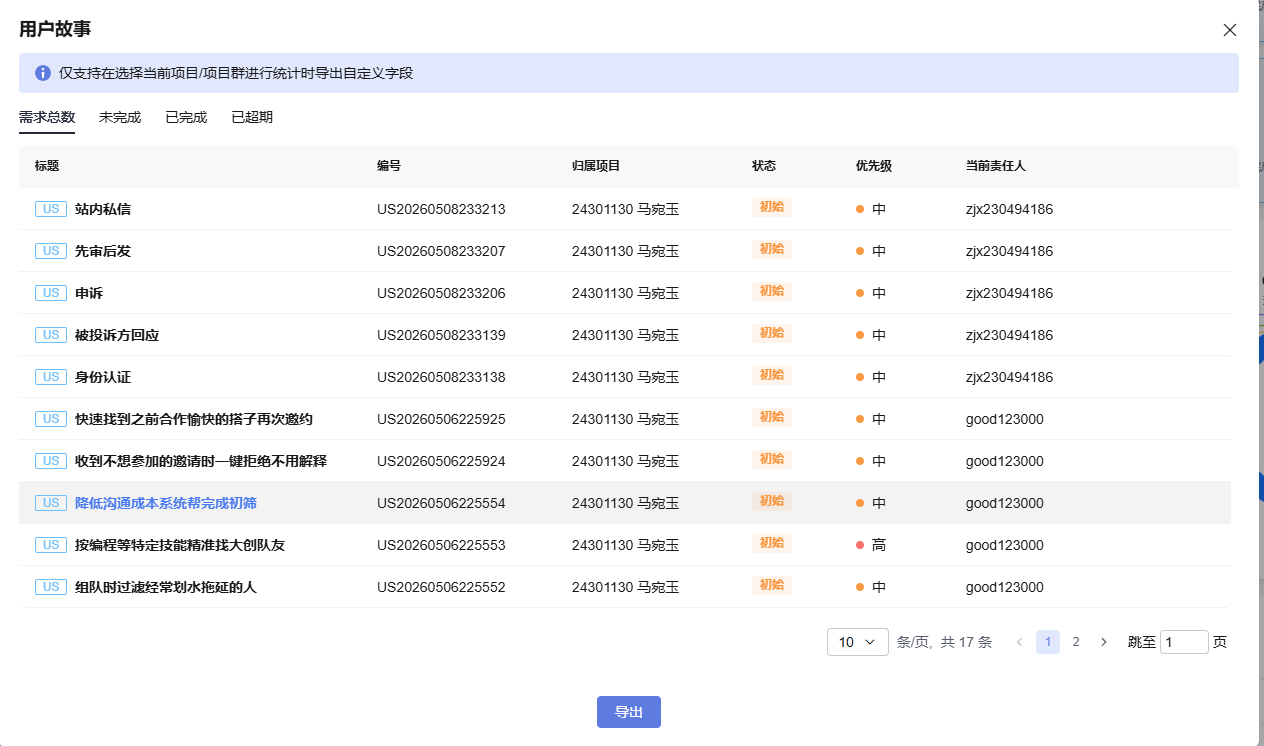
\includegraphics[width=0.96\textwidth,height=0.78\textheight,keepaspectratio]{picture/6-4.png}
\caption{图 6-4 用户故事截图}
\end{figure}

\chapter{7 功能需求详情}\label{ux529fux80fdux9700ux6c42ux8be6ux60c5}

\section{FR-001
校园邮箱登录与身份认证}\label{fr-001-ux6821ux56edux90aeux7bb1ux767bux5f55ux4e0eux8eabux4efdux8ba4ux8bc1}

{\def\LTcaptype{none} % do not increment counter
\begin{xltabular}{\textwidth}{@{}>{\centering\arraybackslash}X>{\centering\arraybackslash}X@{}}
\toprule\noalign{}
\endhead
\bottomrule\noalign{}
\endlastfoot
\textbf{项目} & \textbf{内容} \\
功能编号 & FR-001 \\
功能名称 & 校园邮箱登录与身份认证 \\
所属模块 & 账号与身份认证 \\
适用角色 & 已注册或未注册学生 \\
优先级 & P0 \\
对应用户故事 & US13 \\
\end{xltabular}
}

\subsection{功能描述}\label{ux529fux80fdux63cfux8ff0}

系统支持用户通过校园邮箱验证码完成登录或注册，并提交学号、年级、学院等基础校内信息完成身份认证。认证状态决定发布、邀约、评价和举报等权限。

\subsection{主流程}\label{ux4e3bux6d41ux7a0b}

{\def\LTcaptype{none} % do not increment counter
\begin{xltabular}{\textwidth}{@{}>{\centering\arraybackslash}X>{\centering\arraybackslash}X@{}}
\toprule\noalign{}
\endhead
\bottomrule\noalign{}
\endlastfoot
\textbf{步骤} & \textbf{流程说明} \\
1 & 用户打开软件登录界面。 \\
2 & 输入校园邮箱并获取验证码。 \\
3 & 系统校验验证码，若账号不存在则创建账号。 \\
4 & 用户补充基础校内信息并提交认证。 \\
5 & 系统记录认证状态，认证通过后开放发布和联系权限。 \\
\end{xltabular}
}

\subsection{异常流程}\label{ux5f02ux5e38ux6d41ux7a0b}

\begin{itemize}
\item
  校园邮箱格式错误、验证码错误或过期、学号信息不完整、认证被驳回。
\end{itemize}

\subsection{验收标准}\label{ux9a8cux6536ux6807ux51c6}

\begin{itemize}
\item
  AC-001：邮箱格式合法且验证码正确时，用户可以成功登录。
\item
  AC-002：未完成认证的用户不能发布需求或发起邀约。
\item
  AC-003：认证状态至少包含未认证、认证中、已认证、认证驳回。
\end{itemize}

\section{FR-002
结构化需求发布}\label{fr-002-ux7ed3ux6784ux5316ux9700ux6c42ux53d1ux5e03}

{\def\LTcaptype{none} % do not increment counter
\begin{xltabular}{\textwidth}{@{}>{\centering\arraybackslash}X>{\centering\arraybackslash}X@{}}
\toprule\noalign{}
\endhead
\bottomrule\noalign{}
\endlastfoot
\textbf{项目} & \textbf{内容} \\
功能编号 & FR-002 \\
功能名称 & 结构化需求发布 \\
所属模块 & 需求发布与审核 \\
适用角色 & 已认证学生 \\
优先级 & P0 \\
对应用户故事 & US1、US2、US3、US5、US9 \\
\end{xltabular}
}

\subsection{功能描述}\label{ux529fux80fdux63cfux8ff0-1}

系统应引导用户按场景填写结构化需求信息，避免只发布模糊文字。不同场景可使用不同字段模板，但均需包含标题、场景、时间、地点、人数、标签和补充描述。

\subsection{主流程}\label{ux4e3bux6d41ux7a0b-1}

{\def\LTcaptype{none} % do not increment counter
\begin{xltabular}{\textwidth}{@{}>{\centering\arraybackslash}X>{\centering\arraybackslash}X@{}}
\toprule\noalign{}
\endhead
\bottomrule\noalign{}
\endlastfoot
\textbf{步骤} & \textbf{流程说明} \\
1 & 用户选择发布需求。 \\
2 & 选择场景类型。 \\
3 & 填写时间、地点、人数、标签、要求和描述。 \\
4 & 系统进行必填项和格式校验。 \\
5 & 用户提交后需求进入待审核状态。 \\
\end{xltabular}
}

\subsection{异常流程}\label{ux5f02ux5e38ux6d41ux7a0b-1}

\begin{itemize}
\item
  必填字段为空、时间已过期、人数上限不合理、描述包含违规内容。
\end{itemize}

\subsection{验收标准}\label{ux9a8cux6536ux6807ux51c6-1}

\begin{itemize}
\item
  AC-001：需求提交后状态为待审核，不直接公开。
\item
  AC-002：系统至少提供吃饭、学习、运动等典型场景模板，并支持其他校园搭子邀约场景的发布。
\item
  AC-003：用户可在提交前预览需求内容。
\end{itemize}

\section{FR-003
需求审核与公开展示}\label{fr-003-ux9700ux6c42ux5ba1ux6838ux4e0eux516cux5f00ux5c55ux793a}

{\def\LTcaptype{none} % do not increment counter
\begin{xltabular}{\textwidth}{@{}>{\centering\arraybackslash}X>{\centering\arraybackslash}X@{}}
\toprule\noalign{}
\endhead
\bottomrule\noalign{}
\endlastfoot
\textbf{项目} & \textbf{内容} \\
功能编号 & FR-003 \\
功能名称 & 需求审核与公开展示 \\
所属模块 & 需求发布与审核 / 平台治理 \\
适用角色 & 管理员、需求发布者 \\
优先级 & P0 \\
对应用户故事 & US2、US14 \\
\end{xltabular}
}

\subsection{功能描述}\label{ux529fux80fdux63cfux8ff0-2}

系统应支持管理员对待审核需求进行审核。仅审核通过的需求可进入公开广场；驳回需求需记录原因并通知发布者。

\subsection{主流程}\label{ux4e3bux6d41ux7a0b-2}

{\def\LTcaptype{none} % do not increment counter
\begin{xltabular}{\textwidth}{@{}>{\centering\arraybackslash}X>{\centering\arraybackslash}X@{}}
\toprule\noalign{}
\endhead
\bottomrule\noalign{}
\endlastfoot
\textbf{步骤} & \textbf{流程说明} \\
1 & 管理员进入待审核列表。 \\
2 & 查看需求详情。 \\
3 & 选择通过或驳回并填写审核备注。 \\
4 & 系统更新需求状态。 \\
5 & 通过需求进入广场，驳回需求通知发布者。 \\
\end{xltabular}
}

\subsection{异常流程}\label{ux5f02ux5e38ux6d41ux7a0b-2}

\begin{itemize}
\item
  审核信息不完整、需求被重复提交、管理员误操作。
\end{itemize}

\subsection{验收标准}\label{ux9a8cux6536ux6807ux51c6-2}

\begin{itemize}
\item
  AC-001：需求状态包含草稿、待审核、已发布、已关闭、驳回。
\item
  AC-002：仅已发布需求出现在公开广场。
\item
  AC-003：驳回需求应向发布者展示驳回原因。
\end{itemize}

\section{FR-004
广场浏览、筛选与排序}\label{fr-004-ux5e7fux573aux6d4fux89c8ux7b5bux9009ux4e0eux6392ux5e8f}

{\def\LTcaptype{none} % do not increment counter
\begin{xltabular}{\textwidth}{@{}>{\centering\arraybackslash}X>{\centering\arraybackslash}X@{}}
\toprule\noalign{}
\endhead
\bottomrule\noalign{}
\endlastfoot
\textbf{项目} & \textbf{内容} \\
功能编号 & FR-004 \\
功能名称 & 广场浏览、筛选与排序 \\
所属模块 & 广场发现与筛选 \\
适用角色 & 学生用户 \\
优先级 & P0 \\
对应用户故事 & US1、US3、US5、US10 \\
\end{xltabular}
}

\subsection{功能描述}\label{ux529fux80fdux63cfux8ff0-3}

系统应提供需求广场，用户可按场景、时间、地点、性别、技能/水平、人数、信用摘要等维度筛选，并按时间重合度、地点近似度、发布时间等排序。

\subsection{主流程}\label{ux4e3bux6d41ux7a0b-3}

{\def\LTcaptype{none} % do not increment counter
\begin{xltabular}{\textwidth}{@{}>{\centering\arraybackslash}X>{\centering\arraybackslash}X@{}}
\toprule\noalign{}
\endhead
\bottomrule\noalign{}
\endlastfoot
\textbf{步骤} & \textbf{流程说明} \\
1 & 用户进入广场。 \\
2 & 选择场景和筛选条件。 \\
3 & 系统展示符合条件的需求列表。 \\
4 & 用户进入详情页查看信息。 \\
5 & 用户可发起邀约或收藏/稍后查看。 \\
\end{xltabular}
}

\subsection{异常流程}\label{ux5f02ux5e38ux6d41ux7a0b-3}

\begin{itemize}
\item
  无符合条件结果、筛选条件冲突、需求已关闭但仍被展示。
\end{itemize}

\subsection{验收标准}\label{ux9a8cux6536ux6807ux51c6-3}

\begin{itemize}
\item
  AC-001：用户可以按至少场景、时间、地点三个维度筛选。
\item
  AC-002：已关闭、驳回、待审核需求不得出现在广场。
\item
  AC-003：无结果时应展示清晰的空状态提示。
\end{itemize}

\section{FR-005
邀约与双向确认}\label{fr-005-ux9080ux7ea6ux4e0eux53ccux5411ux786eux8ba4}

{\def\LTcaptype{none} % do not increment counter
\begin{xltabular}{\textwidth}{@{}>{\centering\arraybackslash}X>{\centering\arraybackslash}X@{}}
\toprule\noalign{}
\endhead
\bottomrule\noalign{}
\endlastfoot
\textbf{项目} & \textbf{内容} \\
功能编号 & FR-005 \\
功能名称 & 邀约与双向确认 \\
所属模块 & 邀约与联系确认 \\
适用角色 & 已认证学生、被联系对象 \\
优先级 & P0 \\
对应用户故事 & US7、US11 \\
\end{xltabular}
}

\subsection{功能描述}\label{ux529fux80fdux63cfux8ff0-4}

系统应支持用户从需求详情界面向发布者发起邀约。接收方可接受或拒绝。双方确认前不直接暴露外部联系方式，确认后可进入站内沟通或解锁联系方式。

\subsection{主流程}\label{ux4e3bux6d41ux7a0b-4}

{\def\LTcaptype{none} % do not increment counter
\begin{xltabular}{\textwidth}{@{}>{\centering\arraybackslash}X>{\centering\arraybackslash}X@{}}
\toprule\noalign{}
\endhead
\bottomrule\noalign{}
\endlastfoot
\textbf{步骤} & \textbf{流程说明} \\
1 & 用户查看需求详情。 \\
2 & 点击发起邀约并填写简短留言。 \\
3 & 系统向需求发布者发送邀约通知。 \\
4 & 发布者选择接受或拒绝。 \\
5 & 接受后建立搭子关系并进入沟通/联系方式解锁流程。 \\
\end{xltabular}
}

\subsection{异常流程}\label{ux5f02ux5e38ux6d41ux7a0b-4}

\begin{itemize}
\item
  需求已满员、需求已关闭、重复邀约、被拒绝后反复打扰。
\end{itemize}

\subsection{验收标准}\label{ux9a8cux6536ux6807ux51c6-4}

\begin{itemize}
\item
  AC-001：用户可以从需求详情界面发起邀约。
\item
  AC-002：邀约状态包含已发起、已接受、已拒绝、已失效。
\item
  AC-003：拒绝邀约后系统应提供默认话术并降低后续打扰。
\end{itemize}

\section{FR-006
站内消息与联系方式渐进解锁}\label{fr-006-ux7ad9ux5185ux6d88ux606fux4e0eux8054ux7cfbux65b9ux5f0fux6e10ux8fdbux89e3ux9501}

{\def\LTcaptype{none} % do not increment counter
\begin{xltabular}{\textwidth}{@{}>{\centering\arraybackslash}X>{\centering\arraybackslash}X@{}}
\toprule\noalign{}
\endhead
\bottomrule\noalign{}
\endlastfoot
\textbf{项目} & \textbf{内容} \\
功能编号 & FR-006 \\
功能名称 & 站内消息与联系方式渐进解锁 \\
所属模块 & 邀约与联系确认 \\
适用角色 & 已建立意向双方 \\
优先级 & P1 \\
对应用户故事 & US15 \\
\end{xltabular}
}

\subsection{功能描述}\label{ux529fux80fdux63cfux8ff0-5}

系统应提供轻量站内消息，用于在交换外部联系方式前确认基本情况。站内消息不追求完整
IM 能力，只满足文本、截图和联系方式卡片等基础沟通。

\subsection{主流程}\label{ux4e3bux6d41ux7a0b-5}

{\def\LTcaptype{none} % do not increment counter
\begin{xltabular}{\textwidth}{@{}>{\centering\arraybackslash}X>{\centering\arraybackslash}X@{}}
\toprule\noalign{}
\endhead
\bottomrule\noalign{}
\endlastfoot
\textbf{步骤} & \textbf{流程说明} \\
1 & 双方完成邀约确认。 \\
2 & 系统创建站内会话。 \\
3 & 双方可发送文本或必要截图。 \\
4 & 双方确认后可交换联系方式卡片。 \\
\end{xltabular}
}

\subsection{异常流程}\label{ux5f02ux5e38ux6d41ux7a0b-5}

\begin{itemize}
\item
  恶意消息、联系方式提前泄露、图片内容违规。
\end{itemize}

\subsection{验收标准}\label{ux9a8cux6536ux6807ux51c6-5}

\begin{itemize}
\item
  AC-001：未确认前至少提供一种不直接暴露外部联系方式的联系路径。
\item
  AC-002：联系方式卡片须在双方确认后显示。
\item
  AC-003：用户可对消息或会话发起举报。
\end{itemize}

\section{FR-007
互评与信用摘要}\label{fr-007-ux4e92ux8bc4ux4e0eux4fe1ux7528ux6458ux8981}

{\def\LTcaptype{none} % do not increment counter
\begin{xltabular}{\textwidth}{@{}>{\centering\arraybackslash}X>{\centering\arraybackslash}X@{}}
\toprule\noalign{}
\endhead
\bottomrule\noalign{}
\endlastfoot
\textbf{项目} & \textbf{内容} \\
功能编号 & FR-007 \\
功能名称 & 互评与信用摘要 \\
所属模块 & 评价与信用 \\
适用角色 & 已完成搭子关系双方 \\
优先级 & P1 \\
对应用户故事 & US4、US8 \\
\end{xltabular}
}

\subsection{功能描述}\label{ux529fux80fdux63cfux8ff0-6}

系统应在搭子活动结束后引导双方互评，评价维度包括准时性、合作态度、是否爽约、是否划水等。评价结果形成信用摘要，并作为后续匹配和展示的参考。

\subsection{主流程}\label{ux4e3bux6d41ux7a0b-6}

{\def\LTcaptype{none} % do not increment counter
\begin{xltabular}{\textwidth}{@{}>{\centering\arraybackslash}X>{\centering\arraybackslash}X@{}}
\toprule\noalign{}
\endhead
\bottomrule\noalign{}
\endlastfoot
\textbf{步骤} & \textbf{流程说明} \\
1 & 搭子关系达到完成或关闭条件。 \\
2 & 系统向双方开放评价入口。 \\
3 & 用户填写评分和文字评价。 \\
4 & 系统保存评价并更新信用摘要。 \\
5 & 信用摘要在个人主页或需求详情中适度展示。 \\
\end{xltabular}
}

\subsection{异常流程}\label{ux5f02ux5e38ux6d41ux7a0b-6}

\begin{itemize}
\item
  恶意评价、未合作也评价、评价争议。
\end{itemize}

\subsection{验收标准}\label{ux9a8cux6536ux6807ux51c6-6}

\begin{itemize}
\item
  AC-001：只有存在已确认关系的双方可以互评。
\item
  AC-002：评价维度至少包含准时性和合作态度。
\item
  AC-003：信用摘要可在后续筛选或推荐中作为权重。
\end{itemize}

\section{FR-008
历史搭子记录与再次联系}\label{fr-008-ux5386ux53f2ux642dux5b50ux8bb0ux5f55ux4e0eux518dux6b21ux8054ux7cfb}

{\def\LTcaptype{none} % do not increment counter
\begin{xltabular}{\textwidth}{@{}>{\centering\arraybackslash}X>{\centering\arraybackslash}X@{}}
\toprule\noalign{}
\endhead
\bottomrule\noalign{}
\endlastfoot
\textbf{项目} & \textbf{内容} \\
功能编号 & FR-008 \\
功能名称 & 历史搭子记录与再次联系 \\
所属模块 & 搭子记录与关系管理 \\
适用角色 & 学生用户 \\
优先级 & P1 \\
对应用户故事 & US12 \\
\end{xltabular}
}

\subsection{功能描述}\label{ux529fux80fdux63cfux8ff0-7}

系统应记录用户历史搭子关系，包括场景、时间、对方、评价摘要和完成状态。用户可再次联系历史合作愉快的对象。

\subsection{主流程}\label{ux4e3bux6d41ux7a0b-7}

{\def\LTcaptype{none} % do not increment counter
\begin{xltabular}{\textwidth}{@{}>{\centering\arraybackslash}X>{\centering\arraybackslash}X@{}}
\toprule\noalign{}
\endhead
\bottomrule\noalign{}
\endlastfoot
\textbf{步骤} & \textbf{流程说明} \\
1 & 用户进入个人中心。 \\
2 & 查看历史搭子记录。 \\
3 & 筛选或搜索历史对象。 \\
4 & 选择再次联系或查看评价摘要。 \\
\end{xltabular}
}

\subsection{异常流程}\label{ux5f02ux5e38ux6d41ux7a0b-7}

\begin{itemize}
\item
  历史对象账号被冻结、对方关闭再次联系、记录缺失。
\end{itemize}

\subsection{验收标准}\label{ux9a8cux6536ux6807ux51c6-7}

\begin{itemize}
\item
  AC-001：用户可查看自己参与过的搭子记录。
\item
  AC-002：历史记录包含场景、时间、对方和状态。
\item
  AC-003：再次联系应尊重对方隐私和可联系设置。
\end{itemize}

\section{FR-009
举报、申诉与账号治理}\label{fr-009-ux4e3eux62a5ux7533ux8bc9ux4e0eux8d26ux53f7ux6cbbux7406}

{\def\LTcaptype{none} % do not increment counter
\begin{xltabular}{\textwidth}{@{}>{\centering\arraybackslash}X>{\centering\arraybackslash}X@{}}
\toprule\noalign{}
\endhead
\bottomrule\noalign{}
\endlastfoot
\textbf{项目} & \textbf{内容} \\
功能编号 & FR-009 \\
功能名称 & 举报、申诉与账号治理 \\
所属模块 & 平台治理 \\
适用角色 & 学生用户、管理员 \\
优先级 & P1 \\
对应用户故事 & US16 \\
\end{xltabular}
}

\subsection{功能描述}\label{ux529fux80fdux63cfux8ff0-8}

系统应支持用户对需求、消息、评价或用户进行举报；被处理方可提交申诉并补充证据；管理员对案件进行处理并留痕。

\subsection{主流程}\label{ux4e3bux6d41ux7a0b-8}

{\def\LTcaptype{none} % do not increment counter
\begin{xltabular}{\textwidth}{@{}>{\centering\arraybackslash}X>{\centering\arraybackslash}X@{}}
\toprule\noalign{}
\endhead
\bottomrule\noalign{}
\endlastfoot
\textbf{步骤} & \textbf{流程说明} \\
1 & 用户提交举报或申诉。 \\
2 & 系统生成案件并进入待处理状态。 \\
3 & 管理员查看证据和说明。 \\
4 & 必要时被投诉方补充回应。 \\
5 & 管理员裁定并执行警告、限制、冻结或纠正。 \\
\end{xltabular}
}

\subsection{异常流程}\label{ux5f02ux5e38ux6d41ux7a0b-8}

\begin{itemize}
\item
  恶意举报、证据不足、处理超时、重复申诉。
\end{itemize}

\subsection{验收标准}\label{ux9a8cux6536ux6807ux51c6-8}

\begin{itemize}
\item
  AC-001：案件状态包含待处理、处理中、已裁定、已关闭。
\item
  AC-002：申诉支持文字说明和证据上传。
\item
  AC-003：管理员处理结果需要留痕并可追踪。
\end{itemize}

\chapter{8
界面与交互需求}\label{ux754cux9762ux4e0eux4ea4ux4e92ux9700ux6c42}

\section{8.1 界面清单}\label{ux754cux9762ux6e05ux5355}

{\def\LTcaptype{none} % do not increment counter
\begin{xltabular}{\textwidth}{@{}>{\centering\arraybackslash}X>{\centering\arraybackslash}X>{\centering\arraybackslash}X>{\centering\arraybackslash}X>{\centering\arraybackslash}X@{}}
\toprule\noalign{}
\endhead
\bottomrule\noalign{}
\endlastfoot
\textbf{界面编号} & \textbf{界面名称} & \textbf{界面说明} &
\textbf{适用角色} & \textbf{对应功能} \\
PAGE-001 & 登录 / 注册页 & 校园邮箱验证码登录入口。 & 所有用户 &
FR-001 \\
PAGE-002 & 身份认证界面 & 填写学号、年级、学院等基础校内信息。 &
学生用户 & FR-001 \\
PAGE-003 & 需求发布界面 & 按场景模板填写结构化需求。 & 已认证学生 &
FR-002 \\
PAGE-004 & 需求审核界面 & 管理员查看、通过、驳回待审核需求。 & 管理员 &
FR-003 \\
PAGE-005 & 搭子广场界面 & 浏览、搜索、筛选、排序需求。 & 学生用户 &
FR-004 \\
PAGE-006 & 需求详情界面 & 展示需求详情、发布者信用摘要、发起邀约入口。 &
学生用户 & FR-004 / FR-005 \\
PAGE-007 & 邀约处理界面 & 查看收到的邀约并接受或拒绝。 & 需求发布者 &
FR-005 \\
PAGE-008 & 站内消息界面 & 轻量沟通与联系方式卡片交换。 & 已确认双方 &
FR-006 \\
PAGE-009 & 评价界面 & 完成搭子后进行互评。 & 已完成双方 & FR-007 \\
PAGE-010 & 个人中心界面 &
展示个人资料、认证状态、信用摘要、历史搭子记录。 & 学生用户 & FR-008 \\
PAGE-011 & 举报申诉界面 & 提交举报、申诉，查看处理结果。 & 学生用户 /
管理员 & FR-009 \\
\end{xltabular}
}

\section{8.2
关键交互规则}\label{ux5173ux952eux4ea4ux4e92ux89c4ux5219}

{\def\LTcaptype{none} % do not increment counter
\begin{xltabular}{\textwidth}{@{}>{\centering\arraybackslash}X>{\centering\arraybackslash}X>{\centering\arraybackslash}X>{\centering\arraybackslash}X@{}}
\toprule\noalign{}
\endhead
\bottomrule\noalign{}
\endlastfoot
\textbf{交互编号} & \textbf{触发操作} & \textbf{系统反馈} &
\textbf{备注} \\
UI-001 & 用户提交发布需求 &
若字段完整，提示``已提交审核''；若字段缺失，标出缺失项。 &
避免长篇提示。 \\
UI-002 & 用户筛选广场需求 & 列表实时刷新或点击确认后刷新。 &
优先保证简单清楚。 \\
UI-003 & 用户发起邀约 & 提示``邀约已发送，等待对方确认''。 &
避免直接暴露联系方式。 \\
UI-004 & 对方拒绝邀约 & 向发起方展示温和提示，不显示攻击性信息。 &
降低社交压力。 \\
UI-005 & 需求无匹配结果 & 展示空状态和调整筛选建议。 &
避免用户误以为系统故障。 \\
UI-006 & 评价提交成功 & 提示``评价已提交，将用于信用摘要''。 &
评价后可查看历史记录。 \\
\end{xltabular}
}

\section{8.3
提示文案与错误信息}\label{ux63d0ux793aux6587ux6848ux4e0eux9519ux8befux4fe1ux606f}

{\def\LTcaptype{none} % do not increment counter
\begin{xltabular}{\textwidth}{@{}>{\centering\arraybackslash}X>{\centering\arraybackslash}X>{\centering\arraybackslash}X>{\centering\arraybackslash}X@{}}
\toprule\noalign{}
\endhead
\bottomrule\noalign{}
\endlastfoot
\textbf{场景} & \textbf{提示类型} & \textbf{建议文案} & \textbf{备注} \\
发布成功 & 成功提示 & 需求已提交审核，通过后将在广场展示。 &
强调先审后发。 \\
审核驳回 & 错误提示 & 需求未通过审核，请根据原因修改后重新提交。 &
显示驳回原因。 \\
邀约成功 & 成功提示 & 邀约已发送，请等待对方确认。 & \\
邀约拒绝 & 状态提示 & 对方暂时不方便参与，可以继续寻找其他搭子。 &
避免尴尬。 \\
无筛选结果 & 空状态 & 暂时没有符合条件的搭子，试试放宽时间或地点条件。
& \\
认证未完成 & 权限提示 & 完成校内身份认证后即可发布需求或发起邀约。 & \\
\end{xltabular}
}

\chapter{9 数据需求}\label{ux6570ux636eux9700ux6c42}

\section{9.1
核心数据对象总览}\label{ux6838ux5fc3ux6570ux636eux5bf9ux8c61ux603bux89c8}

{\def\LTcaptype{none} % do not increment counter
\begin{xltabular}{\textwidth}{@{}>{\centering\arraybackslash}X>{\centering\arraybackslash}X>{\centering\arraybackslash}X@{}}
\toprule\noalign{}
\endhead
\bottomrule\noalign{}
\endlastfoot
\textbf{数据对象} & \textbf{关键属性} & \textbf{说明} \\
用户 & 账号状态、认证状态、基础资料、信用摘要、联系方式解锁状态。 &
作为发布者、浏览者、联系方和被联系方的统一主体。 \\
需求 & 场景、标题、描述、时间、地点、人数、状态、标签、审核记录。 &
承载广场发现和联系入口。 \\
邀约 / 会话 &
发起方、接收方、需求、状态、留言、消息内容、联系方式解锁状态。 &
承载低压力联系和渐进确认。 \\
评价 & 评价方、被评价方、维度、分数、文字内容、申诉状态。 &
承载合作后反馈与信用沉淀。 \\
举报 / 申诉案件 & 提交方、对象、说明、证据、被投诉方回应、处理结果。 &
承载治理与纠偏闭环。 \\
\end{xltabular}
}


\section{9.2
数据字段说明}\label{ux6570ux636eux5b57ux6bb5ux8bf4ux660e}

{\def\LTcaptype{none} % do not increment counter
\begin{xltabular}{\textwidth}{@{}>{\centering\arraybackslash}X>{\centering\arraybackslash}X>{\centering\arraybackslash}X>{\centering\arraybackslash}X>{\centering\arraybackslash}X>{\centering\arraybackslash}X@{}}
\toprule\noalign{}
\endhead
\bottomrule\noalign{}
\endlastfoot
\textbf{数据对象} & \textbf{字段名} & \textbf{字段含义} & \textbf{类型}
& \textbf{是否必填} & \textbf{备注} \\
用户 & user\_id & 用户唯一标识 & String/Long & 是 & 系统生成。 \\
用户 & email & 校园邮箱 & String & 是 & 用于登录。 \\
用户 & auth\_status & 认证状态 & Enum & 是 &
未认证、认证中、已认证、认证驳回。 \\
用户 & credit\_summary & 信用摘要 & Object & 否 &
由评价和治理记录汇总。 \\
需求 & demand\_id & 需求唯一标识 & String/Long & 是 & 系统生成。 \\
需求 & scene\_type & 场景类型 & Enum & 是 &
吃饭、学习、运动、小组作业、大创项目。 \\
需求 & title & 需求标题 & String & 是 & 应简洁明确。 \\
需求 & time\_range & 时间范围 & DateTime/Range & 是 &
用于匹配和筛选。 \\
需求 & location & 地点 & String & 是 & 食堂、图书馆、球场等。 \\
需求 & status & 需求状态 & Enum & 是 &
草稿、待审核、已发布、已关闭、驳回。 \\
邀约 & invitation\_id & 邀约唯一标识 & String/Long & 是 & 系统生成。 \\
邀约 & status & 邀约状态 & Enum & 是 &
已发起、已接受、已拒绝、已失效。 \\
评价 & review\_id & 评价唯一标识 & String/Long & 是 & 系统生成。 \\
评价 & punctuality & 准时性评分 & Number & 是 & 信用维度之一。 \\
案件 & case\_status & 案件状态 & Enum & 是 &
待处理、处理中、已裁定、已关闭。 \\
\end{xltabular}
}

\section{9.3
状态流转说明}\label{ux72b6ux6001ux6d41ux8f6cux8bf4ux660e}

{\def\LTcaptype{none} % do not increment counter
\begin{xltabular}{\textwidth}{@{}>{\centering\arraybackslash}X>{\centering\arraybackslash}X>{\centering\arraybackslash}X>{\centering\arraybackslash}X>{\centering\arraybackslash}X@{}}
\toprule\noalign{}
\endhead
\bottomrule\noalign{}
\endlastfoot
\textbf{状态对象} & \textbf{初始状态} & \textbf{中间状态} &
\textbf{终止状态} & \textbf{状态变化规则} \\
用户认证 & 未认证 & 认证中、已认证、认证驳回 & 已认证或认证驳回 &
提交资料后进入认证中，审核通过为已认证，失败为认证驳回。 \\
需求 & 草稿 & 待审核、已发布、驳回 & 已关闭 &
提交后待审核，通过后已发布，用户关闭或过期后已关闭。 \\
邀约 & 已发起 & 已接受、已拒绝 & 已失效 &
接收方接受或拒绝；超时或需求关闭后失效。 \\
案件 & 待处理 & 处理中 & 已裁定、已关闭 &
管理员受理后处理中，裁定后根据是否申诉进入关闭或复核。 \\
\end{xltabular}
}


\chapter{10 非功能需求}\label{ux975eux529fux80fdux9700ux6c42}

\section{10.1 性能需求}\label{ux6027ux80fdux9700ux6c42}

{\def\LTcaptype{none} % do not increment counter
\begin{xltabular}{\textwidth}{@{}>{\centering\arraybackslash}X>{\centering\arraybackslash}X>{\centering\arraybackslash}X>{\centering\arraybackslash}X@{}}
\toprule\noalign{}
\endhead
\bottomrule\noalign{}
\endlastfoot
\textbf{编号} & \textbf{需求项} & \textbf{目标要求} &
\textbf{验证方式} \\
NFR-PERF-001 & 页面响应时间 &
常规页面加载和筛选响应应满足课堂项目可用性要求，避免明显卡顿。 &
功能验证和体验检查。 \\
NFR-PERF-002 & 并发能力 & MVP 阶段至少支持 47 名内测用户同时或高频试用。
& 内测压力模拟。 \\
NFR-PERF-003 & 数据处理能力 & 支持 125
份调研规模基础上扩展到单校学生需求数据。 & 数据量模拟。 \\
\end{xltabular}
}

\section{10.2 安全需求}\label{ux5b89ux5168ux9700ux6c42}

{\def\LTcaptype{none} % do not increment counter
\begin{xltabular}{\textwidth}{@{}>{\centering\arraybackslash}X>{\centering\arraybackslash}X>{\centering\arraybackslash}X>{\centering\arraybackslash}X@{}}
\toprule\noalign{}
\endhead
\bottomrule\noalign{}
\endlastfoot
\textbf{编号} & \textbf{需求项} & \textbf{说明} & \textbf{优先级} \\
NFR-SEC-001 & 身份认证 &
发布、邀约、评价、举报等关键操作需基于登录和校内认证。 & 高 \\
NFR-SEC-002 & 权限控制 &
用户只能编辑本人需求和查看授权范围内的信息；管理员权限单独控制。 & 高 \\
NFR-SEC-003 & 隐私保护 &
联系方式在双方确认前不直接暴露；案件和证据信息限制访问。 & 高 \\
NFR-SEC-004 & 操作日志 & 审核、举报、申诉、冻结等治理动作需要留痕。 &
中 \\
NFR-SEC-005 & 内容安全 &
需求、消息、评价和证据上传需具备基础违规内容处理机制。 & 中 \\
\end{xltabular}
}

\section{10.3 可用性需求}\label{ux53efux7528ux6027ux9700ux6c42}

{\def\LTcaptype{none} % do not increment counter
\begin{xltabular}{\textwidth}{@{}>{\centering\arraybackslash}X>{\centering\arraybackslash}X>{\centering\arraybackslash}X@{}}
\toprule\noalign{}
\endhead
\bottomrule\noalign{}
\endlastfoot
\textbf{编号} & \textbf{需求项} & \textbf{说明} \\
NFR-USE-001 & 少步骤 & 发布、筛选、邀约等关键流程不超过 3
个主要步骤。 \\
NFR-USE-002 & 低学习成本 & 页面结构简单清楚，不需要用户研究复杂规则。 \\
NFR-USE-003 & 明确反馈 & 提交、审核、邀约、评价等动作均提供状态反馈。 \\
NFR-USE-004 & 空状态处理 & 无结果时提供清晰提示和下一步建议。 \\
\end{xltabular}
}

\section{10.4
兼容性与可维护性需求}\label{ux517cux5bb9ux6027ux4e0eux53efux7ef4ux62a4ux6027ux9700ux6c42}

{\def\LTcaptype{none} % do not increment counter
\begin{xltabular}{\textwidth}{@{}>{\centering\arraybackslash}X>{\centering\arraybackslash}X>{\centering\arraybackslash}X@{}}
\toprule\noalign{}
\endhead
\bottomrule\noalign{}
\endlastfoot
\textbf{编号} & \textbf{类型} & \textbf{要求} \\
NFR-COMP-001 & 运行环境兼容 &
软件端应优先兼容主流桌面环境；如采用移动端形态，应保证主流移动设备可正常使用。 \\
NFR-COMP-002 & 设备兼容 & 核心流程应适配电脑和移动端常见运行环境。 \\
NFR-MAIN-001 & 模块化 &
账号、需求、匹配、邀约、评价、治理等模块边界清晰。 \\
NFR-MAIN-002 & 可追踪 & 需求、评价、举报和申诉记录应可查询、可复核。 \\
NFR-MAIN-003 & 可扩展 & 保留多学校、更多场景和推荐规则扩展空间。 \\
\end{xltabular}
}

\chapter{11
约束、假设与依赖}\label{ux7ea6ux675fux5047ux8bbeux4e0eux4f9dux8d56}

\section{11.1 约束条件}\label{ux7ea6ux675fux6761ux4ef6}

{\def\LTcaptype{none} % do not increment counter
\begin{xltabular}{\textwidth}{@{}>{\centering\arraybackslash}X>{\centering\arraybackslash}X>{\centering\arraybackslash}X@{}}
\toprule\noalign{}
\endhead
\bottomrule\noalign{}
\endlastfoot
\textbf{类型} & \textbf{约束说明} & \textbf{影响} \\
时间约束 & 课程项目周期有限，需优先完成可展示、可建模、可验收的主链路。
& P0 优先，避免功能蔓延。 \\
技术约束 & 软件端优先，不开发复杂多端 IM。 &
联系功能以轻量站内消息和联系方式卡片为主。 \\
数据约束 & 当前调研样本集中于单校和部分年级。 & 需求结论更适合单校
MVP。 \\
治理约束 & 管理员处理规则需清晰，否则信用评价可能引发争议。 &
需设计申诉和留痕机制。 \\
隐私约束 & 联系方式、学号、证据材料属于敏感信息。 &
需要权限控制和渐进展示。 \\
\end{xltabular}
}

\section{11.2 假设条件}\label{ux5047ux8bbeux6761ux4ef6}

{\def\LTcaptype{none} % do not increment counter
\begin{xltabular}{\textwidth}{@{}>{\centering\arraybackslash}X>{\centering\arraybackslash}X>{\centering\arraybackslash}X@{}}
\toprule\noalign{}
\endhead
\bottomrule\noalign{}
\endlastfoot
\textbf{编号} & \textbf{假设内容} & \textbf{若不成立的影响} \\
ASM-001 & 学生愿意在平台上填写必要的时间、地点和标签字段。 &
结构化筛选效果下降。 \\
ASM-002 & 校园邮箱或校内信息可作为基础身份认证依据。 &
认证方案需要调整。 \\
ASM-003 & 用户接受匹配后使用微信等外部工具继续沟通。 &
需要增强站内消息能力。 \\
ASM-004 & 47 名愿意内测的学生可支撑 MVP 验证。 &
需要扩大招募或调整验证方式。 \\
\end{xltabular}
}

\section{11.3 依赖项}\label{ux4f9dux8d56ux9879}

{\def\LTcaptype{none} % do not increment counter
\begin{xltabular}{\textwidth}{@{}>{\centering\arraybackslash}X>{\centering\arraybackslash}X>{\centering\arraybackslash}X>{\centering\arraybackslash}X>{\centering\arraybackslash}X@{}}
\toprule\noalign{}
\endhead
\bottomrule\noalign{}
\endlastfoot
\textbf{编号} & \textbf{依赖内容} & \textbf{依赖方} &
\textbf{预计完成时间} & \textbf{风险} \\
DEP-001 & 问卷详细数据和联系方式整理。 & 项目组 & 需求评审后 &
无法联系内测用户。 \\
DEP-002 & 需求管理工具截图。 & 项目组 & 文档提交前 &
截图缺失影响作业要求。 \\
DEP-003 & 用例图、流程图、类图、状态图导出。 & 项目组 & 系统设计前后 &
建模图片缺失影响报告完整性。 \\
DEP-004 & 原型页面或页面草图。 & UI/产品负责人 & 开发前 &
页面需求难以验收。 \\
\end{xltabular}
}

\chapter{12
风险与应对方案}\label{ux98ceux9669ux4e0eux5e94ux5bf9ux65b9ux6848}

{\def\LTcaptype{none} % do not increment counter
\begin{xltabular}{\textwidth}{@{}>{\centering\arraybackslash}X>{\centering\arraybackslash}X>{\centering\arraybackslash}X>{\centering\arraybackslash}X>{\centering\arraybackslash}X>{\centering\arraybackslash}X@{}}
\toprule\noalign{}
\endhead
\bottomrule\noalign{}
\endlastfoot
\textbf{风险编号} & \textbf{风险描述} & \textbf{影响程度} &
\textbf{发生概率} & \textbf{应对方案} & \textbf{负责人} \\
RISK-001 & 用户不愿填写结构化字段，导致发布成本过高。 & 高 & 中 &
控制字段数量，按场景默认模板自动填充可选项。 & 产品负责人 \\
RISK-002 & 内测用户数量不足，匹配池过小。 & 高 & 中 & 优先选择高频 P0
场景，组织定向内测。 & 项目负责人 \\
RISK-003 & 信用评价被恶意使用或引发争议。 & 中 & 中 &
增加申诉、证据、管理员复核和评价展示限制。 & 管理员 \\
RISK-004 & 需求范围扩展到泛社交或完整 IM，导致开发失控。 & 高 & 中 &
坚持产品边界，只做低压力联系和渐进解锁。 & 项目负责人 \\
RISK-005 & 审核和治理流程过重，影响发布效率。 & 中 & 中 & MVP
阶段采用基础审核规则，后续再细化。 & 管理员 \\
RISK-006 & 用户隐私保护不足。 & 高 & 低/中 &
联系方式确认后解锁，证据和案件信息按权限访问。 & 后端负责人 \\
\end{xltabular}
}

\chapter{13 AI 辅助标注}\label{ai-ux8f85ux52a9ux6807ux6ce8}

本需求分析报告初稿的框架设计、内容归纳、表格化整理、语言规范化和部分需求条目补全由生成式人工智能辅助完成，使用工具为
OpenAI ChatGPT（GPT-5.5 Thinking）。AI
辅助内容主要基于项目组提供的问卷报告、访谈纪要、里程碑 1
需求评审材料和已有需求分析草稿。项目组已对以下内容进行人工复核：项目成员信息、课程格式要求、所有截图和建模导出图片、最终需求范围、功能优先级、技术可实现性和最终提交版本。
